\documentclass[twoside]{book}

% Packages required by doxygen
\usepackage{fixltx2e}
\usepackage{calc}
\usepackage{doxygen}
\usepackage[export]{adjustbox} % also loads graphicx
\usepackage{graphicx}
\usepackage[utf8]{inputenc}
\usepackage{makeidx}
\usepackage{multicol}
\usepackage{multirow}
\PassOptionsToPackage{warn}{textcomp}
\usepackage{textcomp}
\usepackage[nointegrals]{wasysym}
\usepackage[table]{xcolor}

% Font selection
\usepackage[T1]{fontenc}
\usepackage[scaled=.90]{helvet}
\usepackage{courier}
\usepackage{amssymb}
\usepackage{sectsty}
\renewcommand{\familydefault}{\sfdefault}
\allsectionsfont{%
  \fontseries{bc}\selectfont%
  \color{darkgray}%
}
\renewcommand{\DoxyLabelFont}{%
  \fontseries{bc}\selectfont%
  \color{darkgray}%
}
\newcommand{\+}{\discretionary{\mbox{\scriptsize$\hookleftarrow$}}{}{}}

% Page & text layout
\usepackage{geometry}
\geometry{%
  a4paper,%
  top=2.5cm,%
  bottom=2.5cm,%
  left=2.5cm,%
  right=2.5cm%
}
\tolerance=750
\hfuzz=15pt
\hbadness=750
\setlength{\emergencystretch}{15pt}
\setlength{\parindent}{0cm}
\setlength{\parskip}{0.2cm}
\makeatletter
\renewcommand{\paragraph}{%
  \@startsection{paragraph}{4}{0ex}{-1.0ex}{1.0ex}{%
    \normalfont\normalsize\bfseries\SS@parafont%
  }%
}
\renewcommand{\subparagraph}{%
  \@startsection{subparagraph}{5}{0ex}{-1.0ex}{1.0ex}{%
    \normalfont\normalsize\bfseries\SS@subparafont%
  }%
}
\makeatother

% Headers & footers
\usepackage{fancyhdr}
\pagestyle{fancyplain}
\fancyhead[LE]{\fancyplain{}{\bfseries\thepage}}
\fancyhead[CE]{\fancyplain{}{}}
\fancyhead[RE]{\fancyplain{}{\bfseries\leftmark}}
\fancyhead[LO]{\fancyplain{}{\bfseries\rightmark}}
\fancyhead[CO]{\fancyplain{}{}}
\fancyhead[RO]{\fancyplain{}{\bfseries\thepage}}
\fancyfoot[LE]{\fancyplain{}{}}
\fancyfoot[CE]{\fancyplain{}{}}
\fancyfoot[RE]{\fancyplain{}{\bfseries\scriptsize Generated on Sun Nov 8 2015 10\+:28\+:36 for Bone Segmentation by Doxygen }}
\fancyfoot[LO]{\fancyplain{}{\bfseries\scriptsize Generated on Sun Nov 8 2015 10\+:28\+:36 for Bone Segmentation by Doxygen }}
\fancyfoot[CO]{\fancyplain{}{}}
\fancyfoot[RO]{\fancyplain{}{}}
\renewcommand{\footrulewidth}{0.4pt}
\renewcommand{\chaptermark}[1]{%
  \markboth{#1}{}%
}
\renewcommand{\sectionmark}[1]{%
  \markright{\thesection\ #1}%
}

% Indices & bibliography
\usepackage{natbib}
\usepackage[titles]{tocloft}
\setcounter{tocdepth}{3}
\setcounter{secnumdepth}{5}
\makeindex

% Hyperlinks (required, but should be loaded last)
\usepackage{ifpdf}
\ifpdf
  \usepackage[pdftex,pagebackref=true]{hyperref}
\else
  \usepackage[ps2pdf,pagebackref=true]{hyperref}
\fi
\hypersetup{%
  colorlinks=true,%
  linkcolor=blue,%
  citecolor=blue,%
  unicode%
}

% Custom commands
\newcommand{\clearemptydoublepage}{%
  \newpage{\pagestyle{empty}\cleardoublepage}%
}


%===== C O N T E N T S =====

\begin{document}

% Titlepage & ToC
\hypersetup{pageanchor=false,
             bookmarks=true,
             bookmarksnumbered=true,
             pdfencoding=unicode
            }
\pagenumbering{roman}
\begin{titlepage}
\vspace*{7cm}
\begin{center}%
{\Large Bone Segmentation }\\
\vspace*{1cm}
{\large Generated by Doxygen 1.8.10}\\
\vspace*{0.5cm}
{\small Sun Nov 8 2015 10:28:36}\\
\end{center}
\end{titlepage}
\clearemptydoublepage
\tableofcontents
\clearemptydoublepage
\pagenumbering{arabic}
\hypersetup{pageanchor=true}

%--- Begin generated contents ---
\chapter{Namespace Index}
\section{Packages}
Here are the packages with brief descriptions (if available)\+:\begin{DoxyCompactList}
\item\contentsline{section}{\hyperlink{namespace_bone_segmentation}{Bone\+Segmentation} }{\pageref{namespace_bone_segmentation}}{}
\item\contentsline{section}{\hyperlink{namespace_markups_info}{Markups\+Info} }{\pageref{namespace_markups_info}}{}
\item\contentsline{section}{\hyperlink{namespacemodule_finder_script}{module\+Finder\+Script} }{\pageref{namespacemodule_finder_script}}{}
\item\contentsline{section}{\hyperlink{namespacesitk_confidence_connected_seg}{sitk\+Confidence\+Connected\+Seg} }{\pageref{namespacesitk_confidence_connected_seg}}{}
\end{DoxyCompactList}

\chapter{Hierarchical Index}
\section{Class Hierarchy}
This inheritance list is sorted roughly, but not completely, alphabetically\+:\begin{DoxyCompactList}
\item \contentsline{section}{Bone\+Segmentation.\+Bone\+Segmentation}{\pageref{class_bone_segmentation_1_1_bone_segmentation}}{}
\item \contentsline{section}{Bone\+Segmentation.\+Bone\+Segmentation\+Logic}{\pageref{class_bone_segmentation_1_1_bone_segmentation_logic}}{}
\item \contentsline{section}{Bone\+Segmentation.\+Bone\+Segmentation\+Widget}{\pageref{class_bone_segmentation_1_1_bone_segmentation_widget}}{}
\item \contentsline{section}{Markups\+Info.\+Markups\+Info}{\pageref{class_markups_info_1_1_markups_info}}{}
\item \contentsline{section}{Markups\+Info.\+Markups\+Info\+Logic}{\pageref{class_markups_info_1_1_markups_info_logic}}{}
\item \contentsline{section}{Markups\+Info.\+Markups\+Info\+Widget}{\pageref{class_markups_info_1_1_markups_info_widget}}{}
\item object\begin{DoxyCompactList}
\item \contentsline{section}{Bone\+Segmentation.\+Slicelet}{\pageref{class_bone_segmentation_1_1_slicelet}}{}
\begin{DoxyCompactList}
\item \contentsline{section}{Bone\+Segmentation.\+Bone\+Segmentation\+Slicelet}{\pageref{class_bone_segmentation_1_1_bone_segmentation_slicelet}}{}
\end{DoxyCompactList}
\end{DoxyCompactList}
\end{DoxyCompactList}

\chapter{Class Index}
\section{Class List}
Here are the classes, structs, unions and interfaces with brief descriptions\+:\begin{DoxyCompactList}
\item\contentsline{section}{\hyperlink{class_bone_segmentation_1_1_bone_segmentation}{Bone\+Segmentation.\+Bone\+Segmentation} }{\pageref{class_bone_segmentation_1_1_bone_segmentation}}{}
\item\contentsline{section}{\hyperlink{class_bone_segmentation_1_1_bone_segmentation_logic}{Bone\+Segmentation.\+Bone\+Segmentation\+Logic} }{\pageref{class_bone_segmentation_1_1_bone_segmentation_logic}}{}
\item\contentsline{section}{\hyperlink{class_bone_segmentation_1_1_bone_segmentation_slicelet}{Bone\+Segmentation.\+Bone\+Segmentation\+Slicelet} }{\pageref{class_bone_segmentation_1_1_bone_segmentation_slicelet}}{}
\item\contentsline{section}{\hyperlink{class_bone_segmentation_1_1_bone_segmentation_widget}{Bone\+Segmentation.\+Bone\+Segmentation\+Widget} }{\pageref{class_bone_segmentation_1_1_bone_segmentation_widget}}{}
\item\contentsline{section}{\hyperlink{class_markups_info_1_1_markups_info}{Markups\+Info.\+Markups\+Info} }{\pageref{class_markups_info_1_1_markups_info}}{}
\item\contentsline{section}{\hyperlink{class_markups_info_1_1_markups_info_logic}{Markups\+Info.\+Markups\+Info\+Logic} }{\pageref{class_markups_info_1_1_markups_info_logic}}{}
\item\contentsline{section}{\hyperlink{class_markups_info_1_1_markups_info_widget}{Markups\+Info.\+Markups\+Info\+Widget} }{\pageref{class_markups_info_1_1_markups_info_widget}}{}
\item\contentsline{section}{\hyperlink{class_bone_segmentation_1_1_slicelet}{Bone\+Segmentation.\+Slicelet} }{\pageref{class_bone_segmentation_1_1_slicelet}}{}
\end{DoxyCompactList}

\chapter{File Index}
\section{File List}
Here is a list of all files with brief descriptions\+:\begin{DoxyCompactList}
\item\contentsline{section}{/\+Users/\+Brent/\+Bone\+Segmentation/\+Slicer\+Module/\+Bone\+Segmentation/\hyperlink{_bone_segmentation_8py}{Bone\+Segmentation.\+py} }{\pageref{_bone_segmentation_8py}}{}
\item\contentsline{section}{/\+Users/\+Brent/\+Bone\+Segmentation/\+Slicer\+Module/\+Bone\+Segmentation/\hyperlink{_markups_info_8py}{Markups\+Info.\+py} }{\pageref{_markups_info_8py}}{}
\item\contentsline{section}{/\+Users/\+Brent/\+Bone\+Segmentation/\+Slicer\+Module/\+Bone\+Segmentation/\hyperlink{module_finder_script_8py}{module\+Finder\+Script.\+py} }{\pageref{module_finder_script_8py}}{}
\item\contentsline{section}{/\+Users/\+Brent/\+Bone\+Segmentation/\+Slicer\+Module/\+Bone\+Segmentation/\hyperlink{sitk_confidence_connected_seg_8py}{sitk\+Confidence\+Connected\+Seg.\+py} }{\pageref{sitk_confidence_connected_seg_8py}}{}
\end{DoxyCompactList}

\chapter{Namespace Documentation}
\hypertarget{namespace_bone_segmentation}{}\section{Bone\+Segmentation Namespace Reference}
\label{namespace_bone_segmentation}\index{Bone\+Segmentation@{Bone\+Segmentation}}
\subsection*{Classes}
\begin{DoxyCompactItemize}
\item 
class \hyperlink{class_bone_segmentation_1_1_bone_segmentation}{Bone\+Segmentation}
\item 
class \hyperlink{class_bone_segmentation_1_1_bone_segmentation_logic}{Bone\+Segmentation\+Logic}
\item 
class \hyperlink{class_bone_segmentation_1_1_bone_segmentation_slicelet}{Bone\+Segmentation\+Slicelet}
\item 
class \hyperlink{class_bone_segmentation_1_1_bone_segmentation_widget}{Bone\+Segmentation\+Widget}
\item 
class \hyperlink{class_bone_segmentation_1_1_slicelet}{Slicelet}
\end{DoxyCompactItemize}
\subsection*{Variables}
\begin{DoxyCompactItemize}
\item 
tuple \hyperlink{namespace_bone_segmentation_abddcab6f9f631fa3e613ecf7a57da568}{slicelet} = \hyperlink{class_bone_segmentation_1_1_bone_segmentation_slicelet}{Bone\+Segmentation\+Slicelet}()
\end{DoxyCompactItemize}


\subsection{Variable Documentation}
\hypertarget{namespace_bone_segmentation_abddcab6f9f631fa3e613ecf7a57da568}{}\index{Bone\+Segmentation@{Bone\+Segmentation}!slicelet@{slicelet}}
\index{slicelet@{slicelet}!Bone\+Segmentation@{Bone\+Segmentation}}
\subsubsection[{slicelet}]{\setlength{\rightskip}{0pt plus 5cm}tuple Bone\+Segmentation.\+slicelet = {\bf Bone\+Segmentation\+Slicelet}()}\label{namespace_bone_segmentation_abddcab6f9f631fa3e613ecf7a57da568}

\hypertarget{namespace_markups_info}{}\section{Markups\+Info Namespace Reference}
\label{namespace_markups_info}\index{Markups\+Info@{Markups\+Info}}
\subsection*{Classes}
\begin{DoxyCompactItemize}
\item 
class \hyperlink{class_markups_info_1_1_markups_info}{Markups\+Info}
\item 
class \hyperlink{class_markups_info_1_1_markups_info_logic}{Markups\+Info\+Logic}
\item 
class \hyperlink{class_markups_info_1_1_markups_info_widget}{Markups\+Info\+Widget}
\end{DoxyCompactItemize}

\hypertarget{namespacemodule_finder_script}{}\section{module\+Finder\+Script Namespace Reference}
\label{namespacemodule_finder_script}\index{module\+Finder\+Script@{module\+Finder\+Script}}
\subsection*{Variables}
\begin{DoxyCompactItemize}
\item 
tuple \hyperlink{namespacemodule_finder_script_a863109df394506ff3b6f1c60c6fcc0a1}{finder} = Module\+Finder()
\end{DoxyCompactItemize}


\subsection{Variable Documentation}
\hypertarget{namespacemodule_finder_script_a863109df394506ff3b6f1c60c6fcc0a1}{}\index{module\+Finder\+Script@{module\+Finder\+Script}!finder@{finder}}
\index{finder@{finder}!module\+Finder\+Script@{module\+Finder\+Script}}
\subsubsection[{finder}]{\setlength{\rightskip}{0pt plus 5cm}tuple module\+Finder\+Script.\+finder = Module\+Finder()}\label{namespacemodule_finder_script_a863109df394506ff3b6f1c60c6fcc0a1}

\hypertarget{namespacesitk_confidence_connected_seg}{}\section{sitk\+Confidence\+Connected\+Seg Namespace Reference}
\label{namespacesitk_confidence_connected_seg}\index{sitk\+Confidence\+Connected\+Seg@{sitk\+Confidence\+Connected\+Seg}}
\subsection*{Functions}
\begin{DoxyCompactItemize}
\item 
def \hyperlink{namespacesitk_confidence_connected_seg_a2be9c5dbc3333db5599c114cae705c89}{Confidence\+Connected\+Seg} (\hyperlink{namespacesitk_confidence_connected_seg_a5013a1ebbf30c96593dd52fe7462750e}{image}, \hyperlink{namespacesitk_confidence_connected_seg_a242f623d43cf8ed6d566b976f4c8ffa4}{seed\+Points})
\end{DoxyCompactItemize}
\subsection*{Variables}
\begin{DoxyCompactItemize}
\item 
list \hyperlink{namespacesitk_confidence_connected_seg_a242f623d43cf8ed6d566b976f4c8ffa4}{seed\+Points} = \mbox{[}\mbox{[}130.\+1238, 184.\+98213, 41.\+123\mbox{]}, \mbox{[}175.\+987, 90.\+123, 31.\+0\mbox{]}\mbox{]}
\item 
tuple \hyperlink{namespacesitk_confidence_connected_seg_a5013a1ebbf30c96593dd52fe7462750e}{image} = sitk.\+Read\+Image(\char`\"{}Volunteer5\+\_\+\+V\+I\+B\+E.\+hdr\char`\"{})
\item 
tuple \hyperlink{namespacesitk_confidence_connected_seg_afc7f0ef969d8d2076c6e7dff1194d1f9}{segmentation} = \hyperlink{namespacesitk_confidence_connected_seg_a2be9c5dbc3333db5599c114cae705c89}{Confidence\+Connected\+Seg}(\hyperlink{namespacesitk_confidence_connected_seg_a5013a1ebbf30c96593dd52fe7462750e}{image}, \hyperlink{namespacesitk_confidence_connected_seg_a242f623d43cf8ed6d566b976f4c8ffa4}{seed\+Points})
\end{DoxyCompactItemize}


\subsection{Function Documentation}
\hypertarget{namespacesitk_confidence_connected_seg_a2be9c5dbc3333db5599c114cae705c89}{}\index{sitk\+Confidence\+Connected\+Seg@{sitk\+Confidence\+Connected\+Seg}!Confidence\+Connected\+Seg@{Confidence\+Connected\+Seg}}
\index{Confidence\+Connected\+Seg@{Confidence\+Connected\+Seg}!sitk\+Confidence\+Connected\+Seg@{sitk\+Confidence\+Connected\+Seg}}
\subsubsection[{Confidence\+Connected\+Seg(image, seed\+Points)}]{\setlength{\rightskip}{0pt plus 5cm}def sitk\+Confidence\+Connected\+Seg.\+Confidence\+Connected\+Seg (
\begin{DoxyParamCaption}
\item[{}]{image, }
\item[{}]{seed\+Points}
\end{DoxyParamCaption}
)}\label{namespacesitk_confidence_connected_seg_a2be9c5dbc3333db5599c114cae705c89}


\subsection{Variable Documentation}
\hypertarget{namespacesitk_confidence_connected_seg_a5013a1ebbf30c96593dd52fe7462750e}{}\index{sitk\+Confidence\+Connected\+Seg@{sitk\+Confidence\+Connected\+Seg}!image@{image}}
\index{image@{image}!sitk\+Confidence\+Connected\+Seg@{sitk\+Confidence\+Connected\+Seg}}
\subsubsection[{image}]{\setlength{\rightskip}{0pt plus 5cm}tuple sitk\+Confidence\+Connected\+Seg.\+image = sitk.\+Read\+Image(\char`\"{}Volunteer5\+\_\+\+V\+I\+B\+E.\+hdr\char`\"{})}\label{namespacesitk_confidence_connected_seg_a5013a1ebbf30c96593dd52fe7462750e}
\hypertarget{namespacesitk_confidence_connected_seg_a242f623d43cf8ed6d566b976f4c8ffa4}{}\index{sitk\+Confidence\+Connected\+Seg@{sitk\+Confidence\+Connected\+Seg}!seed\+Points@{seed\+Points}}
\index{seed\+Points@{seed\+Points}!sitk\+Confidence\+Connected\+Seg@{sitk\+Confidence\+Connected\+Seg}}
\subsubsection[{seed\+Points}]{\setlength{\rightskip}{0pt plus 5cm}list sitk\+Confidence\+Connected\+Seg.\+seed\+Points = \mbox{[}\mbox{[}130.\+1238, 184.\+98213, 41.\+123\mbox{]}, \mbox{[}175.\+987, 90.\+123, 31.\+0\mbox{]}\mbox{]}}\label{namespacesitk_confidence_connected_seg_a242f623d43cf8ed6d566b976f4c8ffa4}
\hypertarget{namespacesitk_confidence_connected_seg_afc7f0ef969d8d2076c6e7dff1194d1f9}{}\index{sitk\+Confidence\+Connected\+Seg@{sitk\+Confidence\+Connected\+Seg}!segmentation@{segmentation}}
\index{segmentation@{segmentation}!sitk\+Confidence\+Connected\+Seg@{sitk\+Confidence\+Connected\+Seg}}
\subsubsection[{segmentation}]{\setlength{\rightskip}{0pt plus 5cm}tuple sitk\+Confidence\+Connected\+Seg.\+segmentation = {\bf Confidence\+Connected\+Seg}({\bf image}, {\bf seed\+Points})}\label{namespacesitk_confidence_connected_seg_afc7f0ef969d8d2076c6e7dff1194d1f9}

\chapter{Class Documentation}
\hypertarget{class_bone_segmentation_1_1_bone_segmentation}{}\section{Bone\+Segmentation.\+Bone\+Segmentation Class Reference}
\label{class_bone_segmentation_1_1_bone_segmentation}\index{Bone\+Segmentation.\+Bone\+Segmentation@{Bone\+Segmentation.\+Bone\+Segmentation}}
\subsection*{Public Member Functions}
\begin{DoxyCompactItemize}
\item 
def \hyperlink{class_bone_segmentation_1_1_bone_segmentation_ad771dd1edcf49a2e3487c4efcf23e857}{\+\_\+\+\_\+init\+\_\+\+\_\+} (self, \hyperlink{class_bone_segmentation_1_1_bone_segmentation_ae7b41133a285837a0054a553cbd40d2c}{parent})
\end{DoxyCompactItemize}
\subsection*{Public Attributes}
\begin{DoxyCompactItemize}
\item 
\hyperlink{class_bone_segmentation_1_1_bone_segmentation_ae7b41133a285837a0054a553cbd40d2c}{parent}
\end{DoxyCompactItemize}


\subsection{Constructor \& Destructor Documentation}
\hypertarget{class_bone_segmentation_1_1_bone_segmentation_ad771dd1edcf49a2e3487c4efcf23e857}{}\index{Bone\+Segmentation\+::\+Bone\+Segmentation@{Bone\+Segmentation\+::\+Bone\+Segmentation}!\+\_\+\+\_\+init\+\_\+\+\_\+@{\+\_\+\+\_\+init\+\_\+\+\_\+}}
\index{\+\_\+\+\_\+init\+\_\+\+\_\+@{\+\_\+\+\_\+init\+\_\+\+\_\+}!Bone\+Segmentation\+::\+Bone\+Segmentation@{Bone\+Segmentation\+::\+Bone\+Segmentation}}
\subsubsection[{\+\_\+\+\_\+init\+\_\+\+\_\+(self, parent)}]{\setlength{\rightskip}{0pt plus 5cm}def Bone\+Segmentation.\+Bone\+Segmentation.\+\_\+\+\_\+init\+\_\+\+\_\+ (
\begin{DoxyParamCaption}
\item[{}]{self, }
\item[{}]{parent}
\end{DoxyParamCaption}
)}\label{class_bone_segmentation_1_1_bone_segmentation_ad771dd1edcf49a2e3487c4efcf23e857}


\subsection{Member Data Documentation}
\hypertarget{class_bone_segmentation_1_1_bone_segmentation_ae7b41133a285837a0054a553cbd40d2c}{}\index{Bone\+Segmentation\+::\+Bone\+Segmentation@{Bone\+Segmentation\+::\+Bone\+Segmentation}!parent@{parent}}
\index{parent@{parent}!Bone\+Segmentation\+::\+Bone\+Segmentation@{Bone\+Segmentation\+::\+Bone\+Segmentation}}
\subsubsection[{parent}]{\setlength{\rightskip}{0pt plus 5cm}Bone\+Segmentation.\+Bone\+Segmentation.\+parent}\label{class_bone_segmentation_1_1_bone_segmentation_ae7b41133a285837a0054a553cbd40d2c}


The documentation for this class was generated from the following file\+:\begin{DoxyCompactItemize}
\item 
/\+Users/\+Brent/\+Bone\+Segmentation/\+Slicer\+Module/\+Bone\+Segmentation/\hyperlink{_bone_segmentation_8py}{Bone\+Segmentation.\+py}\end{DoxyCompactItemize}

\hypertarget{class_bone_segmentation_1_1_bone_segmentation_logic}{}\section{Bone\+Segmentation.\+Bone\+Segmentation\+Logic Class Reference}
\label{class_bone_segmentation_1_1_bone_segmentation_logic}\index{Bone\+Segmentation.\+Bone\+Segmentation\+Logic@{Bone\+Segmentation.\+Bone\+Segmentation\+Logic}}
\subsection*{Public Member Functions}
\begin{DoxyCompactItemize}
\item 
def \hyperlink{class_bone_segmentation_1_1_bone_segmentation_logic_ad0fafb363305a4b4a1c8ea0a87366e35}{\+\_\+\+\_\+init\+\_\+\+\_\+} (self)
\item 
def \hyperlink{class_bone_segmentation_1_1_bone_segmentation_logic_a42be9247b24fb7bb54b13192270a591a}{remove\+Observers} (self)
\item 
def \hyperlink{class_bone_segmentation_1_1_bone_segmentation_logic_a624ecdd90750a0734bf1a4e2f6741b0e}{apply} (self)
\item 
def \hyperlink{class_bone_segmentation_1_1_bone_segmentation_logic_ab8b4b5d13113e270d50180c6df5a1ef8}{auto\+Apply} (self)
\item 
def \hyperlink{class_bone_segmentation_1_1_bone_segmentation_logic_a26d4d3573ca3e18d23f38da1b12bc114}{conditional\+Perform\+Masking}
\item 
def \hyperlink{class_bone_segmentation_1_1_bone_segmentation_logic_a9e1fe441e98bd8645c8f4c0228085f2c}{perform\+Masking}
\end{DoxyCompactItemize}
\subsection*{Public Attributes}
\begin{DoxyCompactItemize}
\item 
\hyperlink{class_bone_segmentation_1_1_bone_segmentation_logic_a7249c35b21308e8010b26106a11e244e}{input\+Volume\+Node}
\item 
\hyperlink{class_bone_segmentation_1_1_bone_segmentation_logic_aa5507f8f268b711b186df8c74a4b9583}{label\+Node}
\item 
\hyperlink{class_bone_segmentation_1_1_bone_segmentation_logic_a2d6bb5dea3368d499007ccfbcc4c1ecc}{output\+Volume\+Node}
\item 
\hyperlink{class_bone_segmentation_1_1_bone_segmentation_logic_a33fd5044dde775bd35d754df789123f1}{observer\+Tags}
\item 
\hyperlink{class_bone_segmentation_1_1_bone_segmentation_logic_ae4725ea90e295cc00dab5cab11a0a646}{last\+Mask\+Label}
\end{DoxyCompactItemize}


\subsection{Detailed Description}
\begin{DoxyVerb}Implement the logic to calculate the mask volume\end{DoxyVerb}
 

\subsection{Constructor \& Destructor Documentation}
\hypertarget{class_bone_segmentation_1_1_bone_segmentation_logic_ad0fafb363305a4b4a1c8ea0a87366e35}{}\index{Bone\+Segmentation\+::\+Bone\+Segmentation\+Logic@{Bone\+Segmentation\+::\+Bone\+Segmentation\+Logic}!\+\_\+\+\_\+init\+\_\+\+\_\+@{\+\_\+\+\_\+init\+\_\+\+\_\+}}
\index{\+\_\+\+\_\+init\+\_\+\+\_\+@{\+\_\+\+\_\+init\+\_\+\+\_\+}!Bone\+Segmentation\+::\+Bone\+Segmentation\+Logic@{Bone\+Segmentation\+::\+Bone\+Segmentation\+Logic}}
\subsubsection[{\+\_\+\+\_\+init\+\_\+\+\_\+(self)}]{\setlength{\rightskip}{0pt plus 5cm}def Bone\+Segmentation.\+Bone\+Segmentation\+Logic.\+\_\+\+\_\+init\+\_\+\+\_\+ (
\begin{DoxyParamCaption}
\item[{}]{self}
\end{DoxyParamCaption}
)}\label{class_bone_segmentation_1_1_bone_segmentation_logic_ad0fafb363305a4b4a1c8ea0a87366e35}


\subsection{Member Function Documentation}
\hypertarget{class_bone_segmentation_1_1_bone_segmentation_logic_a624ecdd90750a0734bf1a4e2f6741b0e}{}\index{Bone\+Segmentation\+::\+Bone\+Segmentation\+Logic@{Bone\+Segmentation\+::\+Bone\+Segmentation\+Logic}!apply@{apply}}
\index{apply@{apply}!Bone\+Segmentation\+::\+Bone\+Segmentation\+Logic@{Bone\+Segmentation\+::\+Bone\+Segmentation\+Logic}}
\subsubsection[{apply(self)}]{\setlength{\rightskip}{0pt plus 5cm}def Bone\+Segmentation.\+Bone\+Segmentation\+Logic.\+apply (
\begin{DoxyParamCaption}
\item[{}]{self}
\end{DoxyParamCaption}
)}\label{class_bone_segmentation_1_1_bone_segmentation_logic_a624ecdd90750a0734bf1a4e2f6741b0e}
\hypertarget{class_bone_segmentation_1_1_bone_segmentation_logic_ab8b4b5d13113e270d50180c6df5a1ef8}{}\index{Bone\+Segmentation\+::\+Bone\+Segmentation\+Logic@{Bone\+Segmentation\+::\+Bone\+Segmentation\+Logic}!auto\+Apply@{auto\+Apply}}
\index{auto\+Apply@{auto\+Apply}!Bone\+Segmentation\+::\+Bone\+Segmentation\+Logic@{Bone\+Segmentation\+::\+Bone\+Segmentation\+Logic}}
\subsubsection[{auto\+Apply(self)}]{\setlength{\rightskip}{0pt plus 5cm}def Bone\+Segmentation.\+Bone\+Segmentation\+Logic.\+auto\+Apply (
\begin{DoxyParamCaption}
\item[{}]{self}
\end{DoxyParamCaption}
)}\label{class_bone_segmentation_1_1_bone_segmentation_logic_ab8b4b5d13113e270d50180c6df5a1ef8}
\hypertarget{class_bone_segmentation_1_1_bone_segmentation_logic_a26d4d3573ca3e18d23f38da1b12bc114}{}\index{Bone\+Segmentation\+::\+Bone\+Segmentation\+Logic@{Bone\+Segmentation\+::\+Bone\+Segmentation\+Logic}!conditional\+Perform\+Masking@{conditional\+Perform\+Masking}}
\index{conditional\+Perform\+Masking@{conditional\+Perform\+Masking}!Bone\+Segmentation\+::\+Bone\+Segmentation\+Logic@{Bone\+Segmentation\+::\+Bone\+Segmentation\+Logic}}
\subsubsection[{conditional\+Perform\+Masking}]{\setlength{\rightskip}{0pt plus 5cm}def Bone\+Segmentation.\+Bone\+Segmentation\+Logic.\+conditional\+Perform\+Masking (
\begin{DoxyParamCaption}
\item[{}]{self, }
\item[{}]{object = {\ttfamily None}, }
\item[{}]{event = {\ttfamily None}}
\end{DoxyParamCaption}
)}\label{class_bone_segmentation_1_1_bone_segmentation_logic_a26d4d3573ca3e18d23f38da1b12bc114}
\begin{DoxyVerb}Since we cannot observe for just the label value
    changing on the parameter node, we check the label value
    or else we would be re-masking for every small edit
    parameter change.\end{DoxyVerb}
 \hypertarget{class_bone_segmentation_1_1_bone_segmentation_logic_a9e1fe441e98bd8645c8f4c0228085f2c}{}\index{Bone\+Segmentation\+::\+Bone\+Segmentation\+Logic@{Bone\+Segmentation\+::\+Bone\+Segmentation\+Logic}!perform\+Masking@{perform\+Masking}}
\index{perform\+Masking@{perform\+Masking}!Bone\+Segmentation\+::\+Bone\+Segmentation\+Logic@{Bone\+Segmentation\+::\+Bone\+Segmentation\+Logic}}
\subsubsection[{perform\+Masking}]{\setlength{\rightskip}{0pt plus 5cm}def Bone\+Segmentation.\+Bone\+Segmentation\+Logic.\+perform\+Masking (
\begin{DoxyParamCaption}
\item[{}]{self, }
\item[{}]{object = {\ttfamily None}, }
\item[{}]{event = {\ttfamily None}}
\end{DoxyParamCaption}
)}\label{class_bone_segmentation_1_1_bone_segmentation_logic_a9e1fe441e98bd8645c8f4c0228085f2c}
\hypertarget{class_bone_segmentation_1_1_bone_segmentation_logic_a42be9247b24fb7bb54b13192270a591a}{}\index{Bone\+Segmentation\+::\+Bone\+Segmentation\+Logic@{Bone\+Segmentation\+::\+Bone\+Segmentation\+Logic}!remove\+Observers@{remove\+Observers}}
\index{remove\+Observers@{remove\+Observers}!Bone\+Segmentation\+::\+Bone\+Segmentation\+Logic@{Bone\+Segmentation\+::\+Bone\+Segmentation\+Logic}}
\subsubsection[{remove\+Observers(self)}]{\setlength{\rightskip}{0pt plus 5cm}def Bone\+Segmentation.\+Bone\+Segmentation\+Logic.\+remove\+Observers (
\begin{DoxyParamCaption}
\item[{}]{self}
\end{DoxyParamCaption}
)}\label{class_bone_segmentation_1_1_bone_segmentation_logic_a42be9247b24fb7bb54b13192270a591a}


\subsection{Member Data Documentation}
\hypertarget{class_bone_segmentation_1_1_bone_segmentation_logic_a7249c35b21308e8010b26106a11e244e}{}\index{Bone\+Segmentation\+::\+Bone\+Segmentation\+Logic@{Bone\+Segmentation\+::\+Bone\+Segmentation\+Logic}!input\+Volume\+Node@{input\+Volume\+Node}}
\index{input\+Volume\+Node@{input\+Volume\+Node}!Bone\+Segmentation\+::\+Bone\+Segmentation\+Logic@{Bone\+Segmentation\+::\+Bone\+Segmentation\+Logic}}
\subsubsection[{input\+Volume\+Node}]{\setlength{\rightskip}{0pt plus 5cm}Bone\+Segmentation.\+Bone\+Segmentation\+Logic.\+input\+Volume\+Node}\label{class_bone_segmentation_1_1_bone_segmentation_logic_a7249c35b21308e8010b26106a11e244e}
\hypertarget{class_bone_segmentation_1_1_bone_segmentation_logic_aa5507f8f268b711b186df8c74a4b9583}{}\index{Bone\+Segmentation\+::\+Bone\+Segmentation\+Logic@{Bone\+Segmentation\+::\+Bone\+Segmentation\+Logic}!label\+Node@{label\+Node}}
\index{label\+Node@{label\+Node}!Bone\+Segmentation\+::\+Bone\+Segmentation\+Logic@{Bone\+Segmentation\+::\+Bone\+Segmentation\+Logic}}
\subsubsection[{label\+Node}]{\setlength{\rightskip}{0pt plus 5cm}Bone\+Segmentation.\+Bone\+Segmentation\+Logic.\+label\+Node}\label{class_bone_segmentation_1_1_bone_segmentation_logic_aa5507f8f268b711b186df8c74a4b9583}
\hypertarget{class_bone_segmentation_1_1_bone_segmentation_logic_ae4725ea90e295cc00dab5cab11a0a646}{}\index{Bone\+Segmentation\+::\+Bone\+Segmentation\+Logic@{Bone\+Segmentation\+::\+Bone\+Segmentation\+Logic}!last\+Mask\+Label@{last\+Mask\+Label}}
\index{last\+Mask\+Label@{last\+Mask\+Label}!Bone\+Segmentation\+::\+Bone\+Segmentation\+Logic@{Bone\+Segmentation\+::\+Bone\+Segmentation\+Logic}}
\subsubsection[{last\+Mask\+Label}]{\setlength{\rightskip}{0pt plus 5cm}Bone\+Segmentation.\+Bone\+Segmentation\+Logic.\+last\+Mask\+Label}\label{class_bone_segmentation_1_1_bone_segmentation_logic_ae4725ea90e295cc00dab5cab11a0a646}
\hypertarget{class_bone_segmentation_1_1_bone_segmentation_logic_a33fd5044dde775bd35d754df789123f1}{}\index{Bone\+Segmentation\+::\+Bone\+Segmentation\+Logic@{Bone\+Segmentation\+::\+Bone\+Segmentation\+Logic}!observer\+Tags@{observer\+Tags}}
\index{observer\+Tags@{observer\+Tags}!Bone\+Segmentation\+::\+Bone\+Segmentation\+Logic@{Bone\+Segmentation\+::\+Bone\+Segmentation\+Logic}}
\subsubsection[{observer\+Tags}]{\setlength{\rightskip}{0pt plus 5cm}Bone\+Segmentation.\+Bone\+Segmentation\+Logic.\+observer\+Tags}\label{class_bone_segmentation_1_1_bone_segmentation_logic_a33fd5044dde775bd35d754df789123f1}
\hypertarget{class_bone_segmentation_1_1_bone_segmentation_logic_a2d6bb5dea3368d499007ccfbcc4c1ecc}{}\index{Bone\+Segmentation\+::\+Bone\+Segmentation\+Logic@{Bone\+Segmentation\+::\+Bone\+Segmentation\+Logic}!output\+Volume\+Node@{output\+Volume\+Node}}
\index{output\+Volume\+Node@{output\+Volume\+Node}!Bone\+Segmentation\+::\+Bone\+Segmentation\+Logic@{Bone\+Segmentation\+::\+Bone\+Segmentation\+Logic}}
\subsubsection[{output\+Volume\+Node}]{\setlength{\rightskip}{0pt plus 5cm}Bone\+Segmentation.\+Bone\+Segmentation\+Logic.\+output\+Volume\+Node}\label{class_bone_segmentation_1_1_bone_segmentation_logic_a2d6bb5dea3368d499007ccfbcc4c1ecc}


The documentation for this class was generated from the following file\+:\begin{DoxyCompactItemize}
\item 
/\+Users/\+Brent/\+Bone\+Segmentation/\+Slicer\+Module/\+Bone\+Segmentation/\hyperlink{_bone_segmentation_8py}{Bone\+Segmentation.\+py}\end{DoxyCompactItemize}

\hypertarget{class_bone_segmentation_1_1_bone_segmentation_slicelet}{}\section{Bone\+Segmentation.\+Bone\+Segmentation\+Slicelet Class Reference}
\label{class_bone_segmentation_1_1_bone_segmentation_slicelet}\index{Bone\+Segmentation.\+Bone\+Segmentation\+Slicelet@{Bone\+Segmentation.\+Bone\+Segmentation\+Slicelet}}
Inheritance diagram for Bone\+Segmentation.\+Bone\+Segmentation\+Slicelet\+:\begin{figure}[H]
\begin{center}
\leavevmode
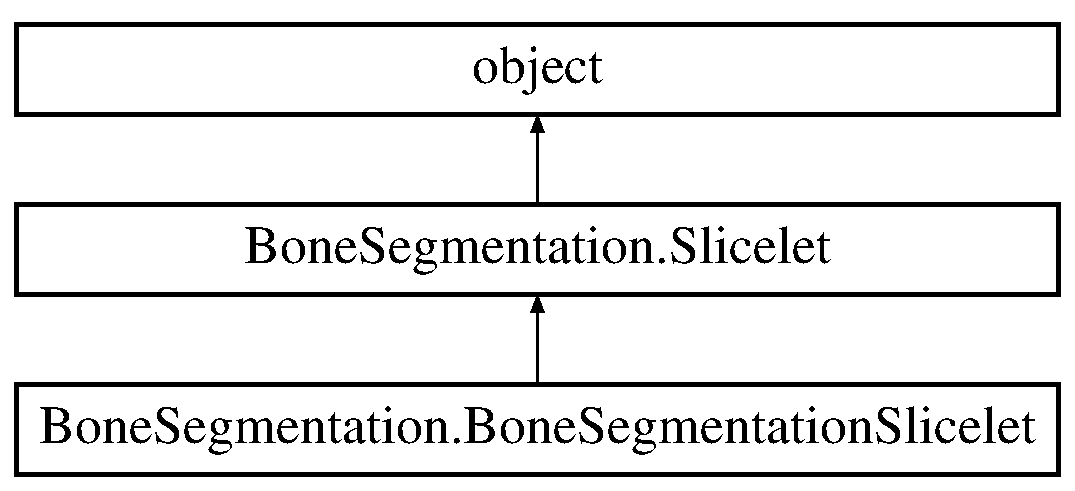
\includegraphics[height=3.000000cm]{class_bone_segmentation_1_1_bone_segmentation_slicelet}
\end{center}
\end{figure}
\subsection*{Public Member Functions}
\begin{DoxyCompactItemize}
\item 
def \hyperlink{class_bone_segmentation_1_1_bone_segmentation_slicelet_a9f410c094d4df3646d6eccf3ba06e22e}{\+\_\+\+\_\+init\+\_\+\+\_\+} (self)
\item 
def \hyperlink{class_bone_segmentation_1_1_bone_segmentation_slicelet_aaf7d20abeae35cdff19660f1d0b2ce20}{enable\+Or\+Disable\+Fiduciale\+Button} (self)
\item 
def \hyperlink{class_bone_segmentation_1_1_bone_segmentation_slicelet_aac05ba6ae75abfd82774e805b5e3720d}{delete\+Fiducials\+Button} (self)
\item 
def \hyperlink{class_bone_segmentation_1_1_bone_segmentation_slicelet_a06dbda3177b62cf4978e1e21cc13b453}{print\+Markers} (self)
\end{DoxyCompactItemize}
\subsection*{Additional Inherited Members}


\subsection{Detailed Description}
\begin{DoxyVerb}Creates the interface when module is run as a stand alone gui app.\end{DoxyVerb}
 

\subsection{Constructor \& Destructor Documentation}
\hypertarget{class_bone_segmentation_1_1_bone_segmentation_slicelet_a9f410c094d4df3646d6eccf3ba06e22e}{}\index{Bone\+Segmentation\+::\+Bone\+Segmentation\+Slicelet@{Bone\+Segmentation\+::\+Bone\+Segmentation\+Slicelet}!\+\_\+\+\_\+init\+\_\+\+\_\+@{\+\_\+\+\_\+init\+\_\+\+\_\+}}
\index{\+\_\+\+\_\+init\+\_\+\+\_\+@{\+\_\+\+\_\+init\+\_\+\+\_\+}!Bone\+Segmentation\+::\+Bone\+Segmentation\+Slicelet@{Bone\+Segmentation\+::\+Bone\+Segmentation\+Slicelet}}
\subsubsection[{\+\_\+\+\_\+init\+\_\+\+\_\+(self)}]{\setlength{\rightskip}{0pt plus 5cm}def Bone\+Segmentation.\+Bone\+Segmentation\+Slicelet.\+\_\+\+\_\+init\+\_\+\+\_\+ (
\begin{DoxyParamCaption}
\item[{}]{self}
\end{DoxyParamCaption}
)}\label{class_bone_segmentation_1_1_bone_segmentation_slicelet_a9f410c094d4df3646d6eccf3ba06e22e}


\subsection{Member Function Documentation}
\hypertarget{class_bone_segmentation_1_1_bone_segmentation_slicelet_aac05ba6ae75abfd82774e805b5e3720d}{}\index{Bone\+Segmentation\+::\+Bone\+Segmentation\+Slicelet@{Bone\+Segmentation\+::\+Bone\+Segmentation\+Slicelet}!delete\+Fiducials\+Button@{delete\+Fiducials\+Button}}
\index{delete\+Fiducials\+Button@{delete\+Fiducials\+Button}!Bone\+Segmentation\+::\+Bone\+Segmentation\+Slicelet@{Bone\+Segmentation\+::\+Bone\+Segmentation\+Slicelet}}
\subsubsection[{delete\+Fiducials\+Button(self)}]{\setlength{\rightskip}{0pt plus 5cm}def Bone\+Segmentation.\+Bone\+Segmentation\+Slicelet.\+delete\+Fiducials\+Button (
\begin{DoxyParamCaption}
\item[{}]{self}
\end{DoxyParamCaption}
)}\label{class_bone_segmentation_1_1_bone_segmentation_slicelet_aac05ba6ae75abfd82774e805b5e3720d}
\hypertarget{class_bone_segmentation_1_1_bone_segmentation_slicelet_aaf7d20abeae35cdff19660f1d0b2ce20}{}\index{Bone\+Segmentation\+::\+Bone\+Segmentation\+Slicelet@{Bone\+Segmentation\+::\+Bone\+Segmentation\+Slicelet}!enable\+Or\+Disable\+Fiduciale\+Button@{enable\+Or\+Disable\+Fiduciale\+Button}}
\index{enable\+Or\+Disable\+Fiduciale\+Button@{enable\+Or\+Disable\+Fiduciale\+Button}!Bone\+Segmentation\+::\+Bone\+Segmentation\+Slicelet@{Bone\+Segmentation\+::\+Bone\+Segmentation\+Slicelet}}
\subsubsection[{enable\+Or\+Disable\+Fiduciale\+Button(self)}]{\setlength{\rightskip}{0pt plus 5cm}def Bone\+Segmentation.\+Bone\+Segmentation\+Slicelet.\+enable\+Or\+Disable\+Fiduciale\+Button (
\begin{DoxyParamCaption}
\item[{}]{self}
\end{DoxyParamCaption}
)}\label{class_bone_segmentation_1_1_bone_segmentation_slicelet_aaf7d20abeae35cdff19660f1d0b2ce20}
\hypertarget{class_bone_segmentation_1_1_bone_segmentation_slicelet_a06dbda3177b62cf4978e1e21cc13b453}{}\index{Bone\+Segmentation\+::\+Bone\+Segmentation\+Slicelet@{Bone\+Segmentation\+::\+Bone\+Segmentation\+Slicelet}!print\+Markers@{print\+Markers}}
\index{print\+Markers@{print\+Markers}!Bone\+Segmentation\+::\+Bone\+Segmentation\+Slicelet@{Bone\+Segmentation\+::\+Bone\+Segmentation\+Slicelet}}
\subsubsection[{print\+Markers(self)}]{\setlength{\rightskip}{0pt plus 5cm}def Bone\+Segmentation.\+Bone\+Segmentation\+Slicelet.\+print\+Markers (
\begin{DoxyParamCaption}
\item[{}]{self}
\end{DoxyParamCaption}
)}\label{class_bone_segmentation_1_1_bone_segmentation_slicelet_a06dbda3177b62cf4978e1e21cc13b453}


The documentation for this class was generated from the following file\+:\begin{DoxyCompactItemize}
\item 
/\+Users/\+Brent/\+Bone\+Segmentation/\+Slicer\+Module/\+Bone\+Segmentation/\hyperlink{_bone_segmentation_8py}{Bone\+Segmentation.\+py}\end{DoxyCompactItemize}

\hypertarget{class_bone_segmentation_1_1_bone_segmentation_widget}{}\section{Bone\+Segmentation.\+Bone\+Segmentation\+Widget Class Reference}
\label{class_bone_segmentation_1_1_bone_segmentation_widget}\index{Bone\+Segmentation.\+Bone\+Segmentation\+Widget@{Bone\+Segmentation.\+Bone\+Segmentation\+Widget}}
\subsection*{Public Member Functions}
\begin{DoxyCompactItemize}
\item 
def \hyperlink{class_bone_segmentation_1_1_bone_segmentation_widget_a7789bc11657d20776e7a8c1f38110e52}{\+\_\+\+\_\+init\+\_\+\+\_\+}
\item 
def \hyperlink{class_bone_segmentation_1_1_bone_segmentation_widget_a4e93b96c69533ee6b76f2320611d559b}{setup} (self)
\item 
def \hyperlink{class_bone_segmentation_1_1_bone_segmentation_widget_a59dd8c955d22afd6cd9a38e6df9886de}{Updatecompute\+Button\+State} (self)
\item 
def \hyperlink{class_bone_segmentation_1_1_bone_segmentation_widget_a9f29ad3fbd78af6166314c5b5bcfbc0b}{on\+Markup\+Select} (self, node)
\item 
def \hyperlink{class_bone_segmentation_1_1_bone_segmentation_widget_a04dff23cd18c96b1501fec0a4d5ff00b}{on\+Compute} (self)
\item 
def \hyperlink{class_bone_segmentation_1_1_bone_segmentation_widget_af5001bcf4f7f4287df81573394d01d03}{update\+Enable\+State} (self)
\item 
def \hyperlink{class_bone_segmentation_1_1_bone_segmentation_widget_a125125e3eae0dfd2724ab384457d1fc2}{on\+Input\+Select} (self, node)
\item 
def \hyperlink{class_bone_segmentation_1_1_bone_segmentation_widget_afa851eebd044552de0aaa8d887e0ab25}{update\+Label\+Text} (self)
\item 
def \hyperlink{class_bone_segmentation_1_1_bone_segmentation_widget_ad0da418d29939cb825a9bc616a883108}{on\+Apply} (self)
\item 
def \hyperlink{class_bone_segmentation_1_1_bone_segmentation_widget_aaa6cceaa3aa1d2a911480b02b1518563}{on\+Auto\+Apply} (self, state)
\end{DoxyCompactItemize}
\subsection*{Public Attributes}
\begin{DoxyCompactItemize}
\item 
\hyperlink{class_bone_segmentation_1_1_bone_segmentation_widget_a0ea50b4a0dff60a3f20d473fa7c5267f}{parent}
\item 
\hyperlink{class_bone_segmentation_1_1_bone_segmentation_widget_a56a110cd069e2b8b28970993cd08a370}{logic}
\item 
\hyperlink{class_bone_segmentation_1_1_bone_segmentation_widget_a6366178a968c7209c01a55f34747c9e0}{Image\+Node}
\item 
\hyperlink{class_bone_segmentation_1_1_bone_segmentation_widget_a2d8eed0881887f1ae1285f8faa855923}{markup\+Selector\+Label}
\item 
\hyperlink{class_bone_segmentation_1_1_bone_segmentation_widget_a6fe4a4a171cf4bf93ed319b694f8f80e}{markup\+Selector}
\item 
\hyperlink{class_bone_segmentation_1_1_bone_segmentation_widget_a087ecc66ea1167394899455299ee3dff}{input\+Volume\+Selector\+Label}
\item 
\hyperlink{class_bone_segmentation_1_1_bone_segmentation_widget_aeef9bc668fa5e4bd4ae83ccae91a52dd}{input\+Selector}
\item 
\hyperlink{class_bone_segmentation_1_1_bone_segmentation_widget_a64c9c6192f80c195649cfd0a575082f9}{compute\+Button}
\item 
\hyperlink{class_bone_segmentation_1_1_bone_segmentation_widget_a753cda86de372958ec7849976a2348f5}{output\+Volume\+Selector\+Label}
\item 
\hyperlink{class_bone_segmentation_1_1_bone_segmentation_widget_abc42def6f122719022ba3a2b1857e5a9}{output\+Selector}
\end{DoxyCompactItemize}


\subsection{Constructor \& Destructor Documentation}
\hypertarget{class_bone_segmentation_1_1_bone_segmentation_widget_a7789bc11657d20776e7a8c1f38110e52}{}\index{Bone\+Segmentation\+::\+Bone\+Segmentation\+Widget@{Bone\+Segmentation\+::\+Bone\+Segmentation\+Widget}!\+\_\+\+\_\+init\+\_\+\+\_\+@{\+\_\+\+\_\+init\+\_\+\+\_\+}}
\index{\+\_\+\+\_\+init\+\_\+\+\_\+@{\+\_\+\+\_\+init\+\_\+\+\_\+}!Bone\+Segmentation\+::\+Bone\+Segmentation\+Widget@{Bone\+Segmentation\+::\+Bone\+Segmentation\+Widget}}
\subsubsection[{\+\_\+\+\_\+init\+\_\+\+\_\+}]{\setlength{\rightskip}{0pt plus 5cm}def Bone\+Segmentation.\+Bone\+Segmentation\+Widget.\+\_\+\+\_\+init\+\_\+\+\_\+ (
\begin{DoxyParamCaption}
\item[{}]{self, }
\item[{}]{parent = {\ttfamily None}}
\end{DoxyParamCaption}
)}\label{class_bone_segmentation_1_1_bone_segmentation_widget_a7789bc11657d20776e7a8c1f38110e52}


\subsection{Member Function Documentation}
\hypertarget{class_bone_segmentation_1_1_bone_segmentation_widget_ad0da418d29939cb825a9bc616a883108}{}\index{Bone\+Segmentation\+::\+Bone\+Segmentation\+Widget@{Bone\+Segmentation\+::\+Bone\+Segmentation\+Widget}!on\+Apply@{on\+Apply}}
\index{on\+Apply@{on\+Apply}!Bone\+Segmentation\+::\+Bone\+Segmentation\+Widget@{Bone\+Segmentation\+::\+Bone\+Segmentation\+Widget}}
\subsubsection[{on\+Apply(self)}]{\setlength{\rightskip}{0pt plus 5cm}def Bone\+Segmentation.\+Bone\+Segmentation\+Widget.\+on\+Apply (
\begin{DoxyParamCaption}
\item[{}]{self}
\end{DoxyParamCaption}
)}\label{class_bone_segmentation_1_1_bone_segmentation_widget_ad0da418d29939cb825a9bc616a883108}
\begin{DoxyVerb}Calculate the mask volume
\end{DoxyVerb}
 \hypertarget{class_bone_segmentation_1_1_bone_segmentation_widget_aaa6cceaa3aa1d2a911480b02b1518563}{}\index{Bone\+Segmentation\+::\+Bone\+Segmentation\+Widget@{Bone\+Segmentation\+::\+Bone\+Segmentation\+Widget}!on\+Auto\+Apply@{on\+Auto\+Apply}}
\index{on\+Auto\+Apply@{on\+Auto\+Apply}!Bone\+Segmentation\+::\+Bone\+Segmentation\+Widget@{Bone\+Segmentation\+::\+Bone\+Segmentation\+Widget}}
\subsubsection[{on\+Auto\+Apply(self, state)}]{\setlength{\rightskip}{0pt plus 5cm}def Bone\+Segmentation.\+Bone\+Segmentation\+Widget.\+on\+Auto\+Apply (
\begin{DoxyParamCaption}
\item[{}]{self, }
\item[{}]{state}
\end{DoxyParamCaption}
)}\label{class_bone_segmentation_1_1_bone_segmentation_widget_aaa6cceaa3aa1d2a911480b02b1518563}
\begin{DoxyVerb}Calculate the mask volume\end{DoxyVerb}
 \hypertarget{class_bone_segmentation_1_1_bone_segmentation_widget_a04dff23cd18c96b1501fec0a4d5ff00b}{}\index{Bone\+Segmentation\+::\+Bone\+Segmentation\+Widget@{Bone\+Segmentation\+::\+Bone\+Segmentation\+Widget}!on\+Compute@{on\+Compute}}
\index{on\+Compute@{on\+Compute}!Bone\+Segmentation\+::\+Bone\+Segmentation\+Widget@{Bone\+Segmentation\+::\+Bone\+Segmentation\+Widget}}
\subsubsection[{on\+Compute(self)}]{\setlength{\rightskip}{0pt plus 5cm}def Bone\+Segmentation.\+Bone\+Segmentation\+Widget.\+on\+Compute (
\begin{DoxyParamCaption}
\item[{}]{self}
\end{DoxyParamCaption}
)}\label{class_bone_segmentation_1_1_bone_segmentation_widget_a04dff23cd18c96b1501fec0a4d5ff00b}
\hypertarget{class_bone_segmentation_1_1_bone_segmentation_widget_a125125e3eae0dfd2724ab384457d1fc2}{}\index{Bone\+Segmentation\+::\+Bone\+Segmentation\+Widget@{Bone\+Segmentation\+::\+Bone\+Segmentation\+Widget}!on\+Input\+Select@{on\+Input\+Select}}
\index{on\+Input\+Select@{on\+Input\+Select}!Bone\+Segmentation\+::\+Bone\+Segmentation\+Widget@{Bone\+Segmentation\+::\+Bone\+Segmentation\+Widget}}
\subsubsection[{on\+Input\+Select(self, node)}]{\setlength{\rightskip}{0pt plus 5cm}def Bone\+Segmentation.\+Bone\+Segmentation\+Widget.\+on\+Input\+Select (
\begin{DoxyParamCaption}
\item[{}]{self, }
\item[{}]{node}
\end{DoxyParamCaption}
)}\label{class_bone_segmentation_1_1_bone_segmentation_widget_a125125e3eae0dfd2724ab384457d1fc2}
\hypertarget{class_bone_segmentation_1_1_bone_segmentation_widget_a9f29ad3fbd78af6166314c5b5bcfbc0b}{}\index{Bone\+Segmentation\+::\+Bone\+Segmentation\+Widget@{Bone\+Segmentation\+::\+Bone\+Segmentation\+Widget}!on\+Markup\+Select@{on\+Markup\+Select}}
\index{on\+Markup\+Select@{on\+Markup\+Select}!Bone\+Segmentation\+::\+Bone\+Segmentation\+Widget@{Bone\+Segmentation\+::\+Bone\+Segmentation\+Widget}}
\subsubsection[{on\+Markup\+Select(self, node)}]{\setlength{\rightskip}{0pt plus 5cm}def Bone\+Segmentation.\+Bone\+Segmentation\+Widget.\+on\+Markup\+Select (
\begin{DoxyParamCaption}
\item[{}]{self, }
\item[{}]{node}
\end{DoxyParamCaption}
)}\label{class_bone_segmentation_1_1_bone_segmentation_widget_a9f29ad3fbd78af6166314c5b5bcfbc0b}
\hypertarget{class_bone_segmentation_1_1_bone_segmentation_widget_a4e93b96c69533ee6b76f2320611d559b}{}\index{Bone\+Segmentation\+::\+Bone\+Segmentation\+Widget@{Bone\+Segmentation\+::\+Bone\+Segmentation\+Widget}!setup@{setup}}
\index{setup@{setup}!Bone\+Segmentation\+::\+Bone\+Segmentation\+Widget@{Bone\+Segmentation\+::\+Bone\+Segmentation\+Widget}}
\subsubsection[{setup(self)}]{\setlength{\rightskip}{0pt plus 5cm}def Bone\+Segmentation.\+Bone\+Segmentation\+Widget.\+setup (
\begin{DoxyParamCaption}
\item[{}]{self}
\end{DoxyParamCaption}
)}\label{class_bone_segmentation_1_1_bone_segmentation_widget_a4e93b96c69533ee6b76f2320611d559b}
\hypertarget{class_bone_segmentation_1_1_bone_segmentation_widget_a59dd8c955d22afd6cd9a38e6df9886de}{}\index{Bone\+Segmentation\+::\+Bone\+Segmentation\+Widget@{Bone\+Segmentation\+::\+Bone\+Segmentation\+Widget}!Updatecompute\+Button\+State@{Updatecompute\+Button\+State}}
\index{Updatecompute\+Button\+State@{Updatecompute\+Button\+State}!Bone\+Segmentation\+::\+Bone\+Segmentation\+Widget@{Bone\+Segmentation\+::\+Bone\+Segmentation\+Widget}}
\subsubsection[{Updatecompute\+Button\+State(self)}]{\setlength{\rightskip}{0pt plus 5cm}def Bone\+Segmentation.\+Bone\+Segmentation\+Widget.\+Updatecompute\+Button\+State (
\begin{DoxyParamCaption}
\item[{}]{self}
\end{DoxyParamCaption}
)}\label{class_bone_segmentation_1_1_bone_segmentation_widget_a59dd8c955d22afd6cd9a38e6df9886de}
\hypertarget{class_bone_segmentation_1_1_bone_segmentation_widget_af5001bcf4f7f4287df81573394d01d03}{}\index{Bone\+Segmentation\+::\+Bone\+Segmentation\+Widget@{Bone\+Segmentation\+::\+Bone\+Segmentation\+Widget}!update\+Enable\+State@{update\+Enable\+State}}
\index{update\+Enable\+State@{update\+Enable\+State}!Bone\+Segmentation\+::\+Bone\+Segmentation\+Widget@{Bone\+Segmentation\+::\+Bone\+Segmentation\+Widget}}
\subsubsection[{update\+Enable\+State(self)}]{\setlength{\rightskip}{0pt plus 5cm}def Bone\+Segmentation.\+Bone\+Segmentation\+Widget.\+update\+Enable\+State (
\begin{DoxyParamCaption}
\item[{}]{self}
\end{DoxyParamCaption}
)}\label{class_bone_segmentation_1_1_bone_segmentation_widget_af5001bcf4f7f4287df81573394d01d03}
\hypertarget{class_bone_segmentation_1_1_bone_segmentation_widget_afa851eebd044552de0aaa8d887e0ab25}{}\index{Bone\+Segmentation\+::\+Bone\+Segmentation\+Widget@{Bone\+Segmentation\+::\+Bone\+Segmentation\+Widget}!update\+Label\+Text@{update\+Label\+Text}}
\index{update\+Label\+Text@{update\+Label\+Text}!Bone\+Segmentation\+::\+Bone\+Segmentation\+Widget@{Bone\+Segmentation\+::\+Bone\+Segmentation\+Widget}}
\subsubsection[{update\+Label\+Text(self)}]{\setlength{\rightskip}{0pt plus 5cm}def Bone\+Segmentation.\+Bone\+Segmentation\+Widget.\+update\+Label\+Text (
\begin{DoxyParamCaption}
\item[{}]{self}
\end{DoxyParamCaption}
)}\label{class_bone_segmentation_1_1_bone_segmentation_widget_afa851eebd044552de0aaa8d887e0ab25}


\subsection{Member Data Documentation}
\hypertarget{class_bone_segmentation_1_1_bone_segmentation_widget_a64c9c6192f80c195649cfd0a575082f9}{}\index{Bone\+Segmentation\+::\+Bone\+Segmentation\+Widget@{Bone\+Segmentation\+::\+Bone\+Segmentation\+Widget}!compute\+Button@{compute\+Button}}
\index{compute\+Button@{compute\+Button}!Bone\+Segmentation\+::\+Bone\+Segmentation\+Widget@{Bone\+Segmentation\+::\+Bone\+Segmentation\+Widget}}
\subsubsection[{compute\+Button}]{\setlength{\rightskip}{0pt plus 5cm}Bone\+Segmentation.\+Bone\+Segmentation\+Widget.\+compute\+Button}\label{class_bone_segmentation_1_1_bone_segmentation_widget_a64c9c6192f80c195649cfd0a575082f9}
\hypertarget{class_bone_segmentation_1_1_bone_segmentation_widget_a6366178a968c7209c01a55f34747c9e0}{}\index{Bone\+Segmentation\+::\+Bone\+Segmentation\+Widget@{Bone\+Segmentation\+::\+Bone\+Segmentation\+Widget}!Image\+Node@{Image\+Node}}
\index{Image\+Node@{Image\+Node}!Bone\+Segmentation\+::\+Bone\+Segmentation\+Widget@{Bone\+Segmentation\+::\+Bone\+Segmentation\+Widget}}
\subsubsection[{Image\+Node}]{\setlength{\rightskip}{0pt plus 5cm}Bone\+Segmentation.\+Bone\+Segmentation\+Widget.\+Image\+Node}\label{class_bone_segmentation_1_1_bone_segmentation_widget_a6366178a968c7209c01a55f34747c9e0}
\hypertarget{class_bone_segmentation_1_1_bone_segmentation_widget_aeef9bc668fa5e4bd4ae83ccae91a52dd}{}\index{Bone\+Segmentation\+::\+Bone\+Segmentation\+Widget@{Bone\+Segmentation\+::\+Bone\+Segmentation\+Widget}!input\+Selector@{input\+Selector}}
\index{input\+Selector@{input\+Selector}!Bone\+Segmentation\+::\+Bone\+Segmentation\+Widget@{Bone\+Segmentation\+::\+Bone\+Segmentation\+Widget}}
\subsubsection[{input\+Selector}]{\setlength{\rightskip}{0pt plus 5cm}Bone\+Segmentation.\+Bone\+Segmentation\+Widget.\+input\+Selector}\label{class_bone_segmentation_1_1_bone_segmentation_widget_aeef9bc668fa5e4bd4ae83ccae91a52dd}
\hypertarget{class_bone_segmentation_1_1_bone_segmentation_widget_a087ecc66ea1167394899455299ee3dff}{}\index{Bone\+Segmentation\+::\+Bone\+Segmentation\+Widget@{Bone\+Segmentation\+::\+Bone\+Segmentation\+Widget}!input\+Volume\+Selector\+Label@{input\+Volume\+Selector\+Label}}
\index{input\+Volume\+Selector\+Label@{input\+Volume\+Selector\+Label}!Bone\+Segmentation\+::\+Bone\+Segmentation\+Widget@{Bone\+Segmentation\+::\+Bone\+Segmentation\+Widget}}
\subsubsection[{input\+Volume\+Selector\+Label}]{\setlength{\rightskip}{0pt plus 5cm}Bone\+Segmentation.\+Bone\+Segmentation\+Widget.\+input\+Volume\+Selector\+Label}\label{class_bone_segmentation_1_1_bone_segmentation_widget_a087ecc66ea1167394899455299ee3dff}
\hypertarget{class_bone_segmentation_1_1_bone_segmentation_widget_a56a110cd069e2b8b28970993cd08a370}{}\index{Bone\+Segmentation\+::\+Bone\+Segmentation\+Widget@{Bone\+Segmentation\+::\+Bone\+Segmentation\+Widget}!logic@{logic}}
\index{logic@{logic}!Bone\+Segmentation\+::\+Bone\+Segmentation\+Widget@{Bone\+Segmentation\+::\+Bone\+Segmentation\+Widget}}
\subsubsection[{logic}]{\setlength{\rightskip}{0pt plus 5cm}Bone\+Segmentation.\+Bone\+Segmentation\+Widget.\+logic}\label{class_bone_segmentation_1_1_bone_segmentation_widget_a56a110cd069e2b8b28970993cd08a370}
\hypertarget{class_bone_segmentation_1_1_bone_segmentation_widget_a6fe4a4a171cf4bf93ed319b694f8f80e}{}\index{Bone\+Segmentation\+::\+Bone\+Segmentation\+Widget@{Bone\+Segmentation\+::\+Bone\+Segmentation\+Widget}!markup\+Selector@{markup\+Selector}}
\index{markup\+Selector@{markup\+Selector}!Bone\+Segmentation\+::\+Bone\+Segmentation\+Widget@{Bone\+Segmentation\+::\+Bone\+Segmentation\+Widget}}
\subsubsection[{markup\+Selector}]{\setlength{\rightskip}{0pt plus 5cm}Bone\+Segmentation.\+Bone\+Segmentation\+Widget.\+markup\+Selector}\label{class_bone_segmentation_1_1_bone_segmentation_widget_a6fe4a4a171cf4bf93ed319b694f8f80e}
\hypertarget{class_bone_segmentation_1_1_bone_segmentation_widget_a2d8eed0881887f1ae1285f8faa855923}{}\index{Bone\+Segmentation\+::\+Bone\+Segmentation\+Widget@{Bone\+Segmentation\+::\+Bone\+Segmentation\+Widget}!markup\+Selector\+Label@{markup\+Selector\+Label}}
\index{markup\+Selector\+Label@{markup\+Selector\+Label}!Bone\+Segmentation\+::\+Bone\+Segmentation\+Widget@{Bone\+Segmentation\+::\+Bone\+Segmentation\+Widget}}
\subsubsection[{markup\+Selector\+Label}]{\setlength{\rightskip}{0pt plus 5cm}Bone\+Segmentation.\+Bone\+Segmentation\+Widget.\+markup\+Selector\+Label}\label{class_bone_segmentation_1_1_bone_segmentation_widget_a2d8eed0881887f1ae1285f8faa855923}
\hypertarget{class_bone_segmentation_1_1_bone_segmentation_widget_abc42def6f122719022ba3a2b1857e5a9}{}\index{Bone\+Segmentation\+::\+Bone\+Segmentation\+Widget@{Bone\+Segmentation\+::\+Bone\+Segmentation\+Widget}!output\+Selector@{output\+Selector}}
\index{output\+Selector@{output\+Selector}!Bone\+Segmentation\+::\+Bone\+Segmentation\+Widget@{Bone\+Segmentation\+::\+Bone\+Segmentation\+Widget}}
\subsubsection[{output\+Selector}]{\setlength{\rightskip}{0pt plus 5cm}Bone\+Segmentation.\+Bone\+Segmentation\+Widget.\+output\+Selector}\label{class_bone_segmentation_1_1_bone_segmentation_widget_abc42def6f122719022ba3a2b1857e5a9}
\hypertarget{class_bone_segmentation_1_1_bone_segmentation_widget_a753cda86de372958ec7849976a2348f5}{}\index{Bone\+Segmentation\+::\+Bone\+Segmentation\+Widget@{Bone\+Segmentation\+::\+Bone\+Segmentation\+Widget}!output\+Volume\+Selector\+Label@{output\+Volume\+Selector\+Label}}
\index{output\+Volume\+Selector\+Label@{output\+Volume\+Selector\+Label}!Bone\+Segmentation\+::\+Bone\+Segmentation\+Widget@{Bone\+Segmentation\+::\+Bone\+Segmentation\+Widget}}
\subsubsection[{output\+Volume\+Selector\+Label}]{\setlength{\rightskip}{0pt plus 5cm}Bone\+Segmentation.\+Bone\+Segmentation\+Widget.\+output\+Volume\+Selector\+Label}\label{class_bone_segmentation_1_1_bone_segmentation_widget_a753cda86de372958ec7849976a2348f5}
\hypertarget{class_bone_segmentation_1_1_bone_segmentation_widget_a0ea50b4a0dff60a3f20d473fa7c5267f}{}\index{Bone\+Segmentation\+::\+Bone\+Segmentation\+Widget@{Bone\+Segmentation\+::\+Bone\+Segmentation\+Widget}!parent@{parent}}
\index{parent@{parent}!Bone\+Segmentation\+::\+Bone\+Segmentation\+Widget@{Bone\+Segmentation\+::\+Bone\+Segmentation\+Widget}}
\subsubsection[{parent}]{\setlength{\rightskip}{0pt plus 5cm}Bone\+Segmentation.\+Bone\+Segmentation\+Widget.\+parent}\label{class_bone_segmentation_1_1_bone_segmentation_widget_a0ea50b4a0dff60a3f20d473fa7c5267f}


The documentation for this class was generated from the following file\+:\begin{DoxyCompactItemize}
\item 
/\+Users/\+Brent/\+Bone\+Segmentation/\+Slicer\+Module/\+Bone\+Segmentation/\hyperlink{_bone_segmentation_8py}{Bone\+Segmentation.\+py}\end{DoxyCompactItemize}

\hypertarget{class_markups_info_1_1_markups_info}{}\section{Markups\+Info.\+Markups\+Info Class Reference}
\label{class_markups_info_1_1_markups_info}\index{Markups\+Info.\+Markups\+Info@{Markups\+Info.\+Markups\+Info}}
\subsection*{Public Member Functions}
\begin{DoxyCompactItemize}
\item 
def \hyperlink{class_markups_info_1_1_markups_info_af32129a122d30314dba4b186b579bcba}{\+\_\+\+\_\+init\+\_\+\+\_\+} (self, \hyperlink{class_markups_info_1_1_markups_info_a6fa903f0e32ab7f1ed35668a4aac5097}{parent})
\end{DoxyCompactItemize}
\subsection*{Public Attributes}
\begin{DoxyCompactItemize}
\item 
\hyperlink{class_markups_info_1_1_markups_info_a6fa903f0e32ab7f1ed35668a4aac5097}{parent}
\end{DoxyCompactItemize}


\subsection{Constructor \& Destructor Documentation}
\hypertarget{class_markups_info_1_1_markups_info_af32129a122d30314dba4b186b579bcba}{}\index{Markups\+Info\+::\+Markups\+Info@{Markups\+Info\+::\+Markups\+Info}!\+\_\+\+\_\+init\+\_\+\+\_\+@{\+\_\+\+\_\+init\+\_\+\+\_\+}}
\index{\+\_\+\+\_\+init\+\_\+\+\_\+@{\+\_\+\+\_\+init\+\_\+\+\_\+}!Markups\+Info\+::\+Markups\+Info@{Markups\+Info\+::\+Markups\+Info}}
\subsubsection[{\+\_\+\+\_\+init\+\_\+\+\_\+(self, parent)}]{\setlength{\rightskip}{0pt plus 5cm}def Markups\+Info.\+Markups\+Info.\+\_\+\+\_\+init\+\_\+\+\_\+ (
\begin{DoxyParamCaption}
\item[{}]{self, }
\item[{}]{parent}
\end{DoxyParamCaption}
)}\label{class_markups_info_1_1_markups_info_af32129a122d30314dba4b186b579bcba}


\subsection{Member Data Documentation}
\hypertarget{class_markups_info_1_1_markups_info_a6fa903f0e32ab7f1ed35668a4aac5097}{}\index{Markups\+Info\+::\+Markups\+Info@{Markups\+Info\+::\+Markups\+Info}!parent@{parent}}
\index{parent@{parent}!Markups\+Info\+::\+Markups\+Info@{Markups\+Info\+::\+Markups\+Info}}
\subsubsection[{parent}]{\setlength{\rightskip}{0pt plus 5cm}Markups\+Info.\+Markups\+Info.\+parent}\label{class_markups_info_1_1_markups_info_a6fa903f0e32ab7f1ed35668a4aac5097}


The documentation for this class was generated from the following file\+:\begin{DoxyCompactItemize}
\item 
/\+Users/\+Brent/\+Bone\+Segmentation/\+Slicer\+Module/\+Bone\+Segmentation/\hyperlink{_markups_info_8py}{Markups\+Info.\+py}\end{DoxyCompactItemize}

\hypertarget{class_markups_info_1_1_markups_info_logic}{}\section{Markups\+Info.\+Markups\+Info\+Logic Class Reference}
\label{class_markups_info_1_1_markups_info_logic}\index{Markups\+Info.\+Markups\+Info\+Logic@{Markups\+Info.\+Markups\+Info\+Logic}}
\subsection*{Public Member Functions}
\begin{DoxyCompactItemize}
\item 
def \hyperlink{class_markups_info_1_1_markups_info_logic_a2a84df484074c4c6914ea564dba4bc7e}{\+\_\+\+\_\+init\+\_\+\+\_\+} (self, markup\+Node)
\end{DoxyCompactItemize}
\subsection*{Public Attributes}
\begin{DoxyCompactItemize}
\item 
\hyperlink{class_markups_info_1_1_markups_info_logic_a6686b8ed0153b4d5c210ae7bfa1a174e}{info}
\end{DoxyCompactItemize}


\subsection{Detailed Description}
\begin{DoxyVerb}Implement the logic to compute markup info
Nodes are passed in as arguments.
Results are stored as 'info' instance variable.
\end{DoxyVerb}
 

\subsection{Constructor \& Destructor Documentation}
\hypertarget{class_markups_info_1_1_markups_info_logic_a2a84df484074c4c6914ea564dba4bc7e}{}\index{Markups\+Info\+::\+Markups\+Info\+Logic@{Markups\+Info\+::\+Markups\+Info\+Logic}!\+\_\+\+\_\+init\+\_\+\+\_\+@{\+\_\+\+\_\+init\+\_\+\+\_\+}}
\index{\+\_\+\+\_\+init\+\_\+\+\_\+@{\+\_\+\+\_\+init\+\_\+\+\_\+}!Markups\+Info\+::\+Markups\+Info\+Logic@{Markups\+Info\+::\+Markups\+Info\+Logic}}
\subsubsection[{\+\_\+\+\_\+init\+\_\+\+\_\+(self, markup\+Node)}]{\setlength{\rightskip}{0pt plus 5cm}def Markups\+Info.\+Markups\+Info\+Logic.\+\_\+\+\_\+init\+\_\+\+\_\+ (
\begin{DoxyParamCaption}
\item[{}]{self, }
\item[{}]{markup\+Node}
\end{DoxyParamCaption}
)}\label{class_markups_info_1_1_markups_info_logic_a2a84df484074c4c6914ea564dba4bc7e}


\subsection{Member Data Documentation}
\hypertarget{class_markups_info_1_1_markups_info_logic_a6686b8ed0153b4d5c210ae7bfa1a174e}{}\index{Markups\+Info\+::\+Markups\+Info\+Logic@{Markups\+Info\+::\+Markups\+Info\+Logic}!info@{info}}
\index{info@{info}!Markups\+Info\+::\+Markups\+Info\+Logic@{Markups\+Info\+::\+Markups\+Info\+Logic}}
\subsubsection[{info}]{\setlength{\rightskip}{0pt plus 5cm}Markups\+Info.\+Markups\+Info\+Logic.\+info}\label{class_markups_info_1_1_markups_info_logic_a6686b8ed0153b4d5c210ae7bfa1a174e}


The documentation for this class was generated from the following file\+:\begin{DoxyCompactItemize}
\item 
/\+Users/\+Brent/\+Bone\+Segmentation/\+Slicer\+Module/\+Bone\+Segmentation/\hyperlink{_markups_info_8py}{Markups\+Info.\+py}\end{DoxyCompactItemize}

\hypertarget{class_markups_info_1_1_markups_info_widget}{}\section{Markups\+Info.\+Markups\+Info\+Widget Class Reference}
\label{class_markups_info_1_1_markups_info_widget}\index{Markups\+Info.\+Markups\+Info\+Widget@{Markups\+Info.\+Markups\+Info\+Widget}}
\subsection*{Public Member Functions}
\begin{DoxyCompactItemize}
\item 
def \hyperlink{class_markups_info_1_1_markups_info_widget_a8231d2418ff192e62e62361b62358568}{\+\_\+\+\_\+init\+\_\+\+\_\+}
\item 
def \hyperlink{class_markups_info_1_1_markups_info_widget_adca013554e00da47c992ce8df6ca530b}{setup} (self)
\item 
def \hyperlink{class_markups_info_1_1_markups_info_widget_a11cd87de1fc9227e6d72092c3acb6787}{Updatecompute\+Button\+State} (self)
\item 
def \hyperlink{class_markups_info_1_1_markups_info_widget_a723ba32aeb870784b2beeffa387fa500}{on\+Markup\+Select} (self, node)
\item 
def \hyperlink{class_markups_info_1_1_markups_info_widget_acf36666a3ce7e86e2d4e433f4ddc8560}{on\+Compute} (self)
\end{DoxyCompactItemize}
\subsection*{Public Attributes}
\begin{DoxyCompactItemize}
\item 
\hyperlink{class_markups_info_1_1_markups_info_widget_ad3681dfadf34f6b646e092e626c02269}{parent}
\item 
\hyperlink{class_markups_info_1_1_markups_info_widget_a90719607e3574542aef2f4fbc8b38694}{logic}
\item 
\hyperlink{class_markups_info_1_1_markups_info_widget_ac603f15c61bd6cb65c949f2f7d151c17}{markup\+Selector\+Label}
\item 
\hyperlink{class_markups_info_1_1_markups_info_widget_aa3adfbb4f342bf9e3063613cf29c6808}{markup\+Selector}
\item 
\hyperlink{class_markups_info_1_1_markups_info_widget_a7ed23a4ba5f19534f7addab2d8d0a63f}{compute\+Button}
\item 
\hyperlink{class_markups_info_1_1_markups_info_widget_af5845a2231b4de465af8658e1e5039df}{total\+Distance\+Label}
\item 
\hyperlink{class_markups_info_1_1_markups_info_widget_ac2b547cb4aadcf3f29c37392d3f0d8b8}{total\+Distance\+Value}
\end{DoxyCompactItemize}


\subsection{Constructor \& Destructor Documentation}
\hypertarget{class_markups_info_1_1_markups_info_widget_a8231d2418ff192e62e62361b62358568}{}\index{Markups\+Info\+::\+Markups\+Info\+Widget@{Markups\+Info\+::\+Markups\+Info\+Widget}!\+\_\+\+\_\+init\+\_\+\+\_\+@{\+\_\+\+\_\+init\+\_\+\+\_\+}}
\index{\+\_\+\+\_\+init\+\_\+\+\_\+@{\+\_\+\+\_\+init\+\_\+\+\_\+}!Markups\+Info\+::\+Markups\+Info\+Widget@{Markups\+Info\+::\+Markups\+Info\+Widget}}
\subsubsection[{\+\_\+\+\_\+init\+\_\+\+\_\+}]{\setlength{\rightskip}{0pt plus 5cm}def Markups\+Info.\+Markups\+Info\+Widget.\+\_\+\+\_\+init\+\_\+\+\_\+ (
\begin{DoxyParamCaption}
\item[{}]{self, }
\item[{}]{parent = {\ttfamily None}}
\end{DoxyParamCaption}
)}\label{class_markups_info_1_1_markups_info_widget_a8231d2418ff192e62e62361b62358568}


\subsection{Member Function Documentation}
\hypertarget{class_markups_info_1_1_markups_info_widget_acf36666a3ce7e86e2d4e433f4ddc8560}{}\index{Markups\+Info\+::\+Markups\+Info\+Widget@{Markups\+Info\+::\+Markups\+Info\+Widget}!on\+Compute@{on\+Compute}}
\index{on\+Compute@{on\+Compute}!Markups\+Info\+::\+Markups\+Info\+Widget@{Markups\+Info\+::\+Markups\+Info\+Widget}}
\subsubsection[{on\+Compute(self)}]{\setlength{\rightskip}{0pt plus 5cm}def Markups\+Info.\+Markups\+Info\+Widget.\+on\+Compute (
\begin{DoxyParamCaption}
\item[{}]{self}
\end{DoxyParamCaption}
)}\label{class_markups_info_1_1_markups_info_widget_acf36666a3ce7e86e2d4e433f4ddc8560}
\hypertarget{class_markups_info_1_1_markups_info_widget_a723ba32aeb870784b2beeffa387fa500}{}\index{Markups\+Info\+::\+Markups\+Info\+Widget@{Markups\+Info\+::\+Markups\+Info\+Widget}!on\+Markup\+Select@{on\+Markup\+Select}}
\index{on\+Markup\+Select@{on\+Markup\+Select}!Markups\+Info\+::\+Markups\+Info\+Widget@{Markups\+Info\+::\+Markups\+Info\+Widget}}
\subsubsection[{on\+Markup\+Select(self, node)}]{\setlength{\rightskip}{0pt plus 5cm}def Markups\+Info.\+Markups\+Info\+Widget.\+on\+Markup\+Select (
\begin{DoxyParamCaption}
\item[{}]{self, }
\item[{}]{node}
\end{DoxyParamCaption}
)}\label{class_markups_info_1_1_markups_info_widget_a723ba32aeb870784b2beeffa387fa500}
\hypertarget{class_markups_info_1_1_markups_info_widget_adca013554e00da47c992ce8df6ca530b}{}\index{Markups\+Info\+::\+Markups\+Info\+Widget@{Markups\+Info\+::\+Markups\+Info\+Widget}!setup@{setup}}
\index{setup@{setup}!Markups\+Info\+::\+Markups\+Info\+Widget@{Markups\+Info\+::\+Markups\+Info\+Widget}}
\subsubsection[{setup(self)}]{\setlength{\rightskip}{0pt plus 5cm}def Markups\+Info.\+Markups\+Info\+Widget.\+setup (
\begin{DoxyParamCaption}
\item[{}]{self}
\end{DoxyParamCaption}
)}\label{class_markups_info_1_1_markups_info_widget_adca013554e00da47c992ce8df6ca530b}
\hypertarget{class_markups_info_1_1_markups_info_widget_a11cd87de1fc9227e6d72092c3acb6787}{}\index{Markups\+Info\+::\+Markups\+Info\+Widget@{Markups\+Info\+::\+Markups\+Info\+Widget}!Updatecompute\+Button\+State@{Updatecompute\+Button\+State}}
\index{Updatecompute\+Button\+State@{Updatecompute\+Button\+State}!Markups\+Info\+::\+Markups\+Info\+Widget@{Markups\+Info\+::\+Markups\+Info\+Widget}}
\subsubsection[{Updatecompute\+Button\+State(self)}]{\setlength{\rightskip}{0pt plus 5cm}def Markups\+Info.\+Markups\+Info\+Widget.\+Updatecompute\+Button\+State (
\begin{DoxyParamCaption}
\item[{}]{self}
\end{DoxyParamCaption}
)}\label{class_markups_info_1_1_markups_info_widget_a11cd87de1fc9227e6d72092c3acb6787}


\subsection{Member Data Documentation}
\hypertarget{class_markups_info_1_1_markups_info_widget_a7ed23a4ba5f19534f7addab2d8d0a63f}{}\index{Markups\+Info\+::\+Markups\+Info\+Widget@{Markups\+Info\+::\+Markups\+Info\+Widget}!compute\+Button@{compute\+Button}}
\index{compute\+Button@{compute\+Button}!Markups\+Info\+::\+Markups\+Info\+Widget@{Markups\+Info\+::\+Markups\+Info\+Widget}}
\subsubsection[{compute\+Button}]{\setlength{\rightskip}{0pt plus 5cm}Markups\+Info.\+Markups\+Info\+Widget.\+compute\+Button}\label{class_markups_info_1_1_markups_info_widget_a7ed23a4ba5f19534f7addab2d8d0a63f}
\hypertarget{class_markups_info_1_1_markups_info_widget_a90719607e3574542aef2f4fbc8b38694}{}\index{Markups\+Info\+::\+Markups\+Info\+Widget@{Markups\+Info\+::\+Markups\+Info\+Widget}!logic@{logic}}
\index{logic@{logic}!Markups\+Info\+::\+Markups\+Info\+Widget@{Markups\+Info\+::\+Markups\+Info\+Widget}}
\subsubsection[{logic}]{\setlength{\rightskip}{0pt plus 5cm}Markups\+Info.\+Markups\+Info\+Widget.\+logic}\label{class_markups_info_1_1_markups_info_widget_a90719607e3574542aef2f4fbc8b38694}
\hypertarget{class_markups_info_1_1_markups_info_widget_aa3adfbb4f342bf9e3063613cf29c6808}{}\index{Markups\+Info\+::\+Markups\+Info\+Widget@{Markups\+Info\+::\+Markups\+Info\+Widget}!markup\+Selector@{markup\+Selector}}
\index{markup\+Selector@{markup\+Selector}!Markups\+Info\+::\+Markups\+Info\+Widget@{Markups\+Info\+::\+Markups\+Info\+Widget}}
\subsubsection[{markup\+Selector}]{\setlength{\rightskip}{0pt plus 5cm}Markups\+Info.\+Markups\+Info\+Widget.\+markup\+Selector}\label{class_markups_info_1_1_markups_info_widget_aa3adfbb4f342bf9e3063613cf29c6808}
\hypertarget{class_markups_info_1_1_markups_info_widget_ac603f15c61bd6cb65c949f2f7d151c17}{}\index{Markups\+Info\+::\+Markups\+Info\+Widget@{Markups\+Info\+::\+Markups\+Info\+Widget}!markup\+Selector\+Label@{markup\+Selector\+Label}}
\index{markup\+Selector\+Label@{markup\+Selector\+Label}!Markups\+Info\+::\+Markups\+Info\+Widget@{Markups\+Info\+::\+Markups\+Info\+Widget}}
\subsubsection[{markup\+Selector\+Label}]{\setlength{\rightskip}{0pt plus 5cm}Markups\+Info.\+Markups\+Info\+Widget.\+markup\+Selector\+Label}\label{class_markups_info_1_1_markups_info_widget_ac603f15c61bd6cb65c949f2f7d151c17}
\hypertarget{class_markups_info_1_1_markups_info_widget_ad3681dfadf34f6b646e092e626c02269}{}\index{Markups\+Info\+::\+Markups\+Info\+Widget@{Markups\+Info\+::\+Markups\+Info\+Widget}!parent@{parent}}
\index{parent@{parent}!Markups\+Info\+::\+Markups\+Info\+Widget@{Markups\+Info\+::\+Markups\+Info\+Widget}}
\subsubsection[{parent}]{\setlength{\rightskip}{0pt plus 5cm}Markups\+Info.\+Markups\+Info\+Widget.\+parent}\label{class_markups_info_1_1_markups_info_widget_ad3681dfadf34f6b646e092e626c02269}
\hypertarget{class_markups_info_1_1_markups_info_widget_af5845a2231b4de465af8658e1e5039df}{}\index{Markups\+Info\+::\+Markups\+Info\+Widget@{Markups\+Info\+::\+Markups\+Info\+Widget}!total\+Distance\+Label@{total\+Distance\+Label}}
\index{total\+Distance\+Label@{total\+Distance\+Label}!Markups\+Info\+::\+Markups\+Info\+Widget@{Markups\+Info\+::\+Markups\+Info\+Widget}}
\subsubsection[{total\+Distance\+Label}]{\setlength{\rightskip}{0pt plus 5cm}Markups\+Info.\+Markups\+Info\+Widget.\+total\+Distance\+Label}\label{class_markups_info_1_1_markups_info_widget_af5845a2231b4de465af8658e1e5039df}
\hypertarget{class_markups_info_1_1_markups_info_widget_ac2b547cb4aadcf3f29c37392d3f0d8b8}{}\index{Markups\+Info\+::\+Markups\+Info\+Widget@{Markups\+Info\+::\+Markups\+Info\+Widget}!total\+Distance\+Value@{total\+Distance\+Value}}
\index{total\+Distance\+Value@{total\+Distance\+Value}!Markups\+Info\+::\+Markups\+Info\+Widget@{Markups\+Info\+::\+Markups\+Info\+Widget}}
\subsubsection[{total\+Distance\+Value}]{\setlength{\rightskip}{0pt plus 5cm}Markups\+Info.\+Markups\+Info\+Widget.\+total\+Distance\+Value}\label{class_markups_info_1_1_markups_info_widget_ac2b547cb4aadcf3f29c37392d3f0d8b8}


The documentation for this class was generated from the following file\+:\begin{DoxyCompactItemize}
\item 
/\+Users/\+Brent/\+Bone\+Segmentation/\+Slicer\+Module/\+Bone\+Segmentation/\hyperlink{_markups_info_8py}{Markups\+Info.\+py}\end{DoxyCompactItemize}

\hypertarget{class_bone_segmentation_1_1_slicelet}{}\section{Bone\+Segmentation.\+Slicelet Class Reference}
\label{class_bone_segmentation_1_1_slicelet}\index{Bone\+Segmentation.\+Slicelet@{Bone\+Segmentation.\+Slicelet}}
Inheritance diagram for Bone\+Segmentation.\+Slicelet\+:\begin{figure}[H]
\begin{center}
\leavevmode
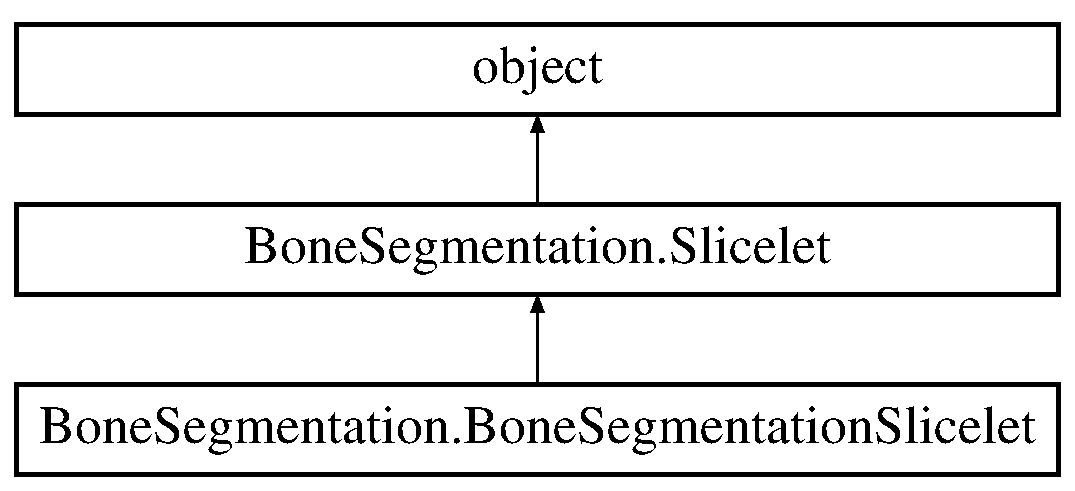
\includegraphics[height=3.000000cm]{class_bone_segmentation_1_1_slicelet}
\end{center}
\end{figure}
\subsection*{Public Member Functions}
\begin{DoxyCompactItemize}
\item 
def \hyperlink{class_bone_segmentation_1_1_slicelet_a9a52cc43bcdb068afd75c64af5df2dd3}{\+\_\+\+\_\+init\+\_\+\+\_\+}
\end{DoxyCompactItemize}
\subsection*{Public Attributes}
\begin{DoxyCompactItemize}
\item 
\hyperlink{class_bone_segmentation_1_1_slicelet_aca71eb02d750fd28af4b5c154ff243af}{parent}
\item 
\hyperlink{class_bone_segmentation_1_1_slicelet_af664e9fb7102f143122def489d7274ba}{buttons}
\item 
\hyperlink{class_bone_segmentation_1_1_slicelet_ac817c61a0c0ebd93996cf88c7a0e993f}{add\+Data\+Button}
\item 
\hyperlink{class_bone_segmentation_1_1_slicelet_ad6a6e46817322b3e798bd1f0bf4e1517}{load\+Scene\+Button}
\item 
\hyperlink{class_bone_segmentation_1_1_slicelet_ac7a8c45c28db3f0ec392fa1a3ece82e4}{buttons\+Col\+Two}
\item 
\hyperlink{class_bone_segmentation_1_1_slicelet_a3024a9863f8c9717ccdd8f3d240d6a5c}{add\+Marker\+Button}
\item 
\hyperlink{class_bone_segmentation_1_1_slicelet_ae426d40722b7369c63d394bcebc10a9c}{delete\+Marker\+Button}
\item 
\hyperlink{class_bone_segmentation_1_1_slicelet_aa21581cbef1468a9b9227cde81133580}{print\+Markers\+Button}
\item 
\hyperlink{class_bone_segmentation_1_1_slicelet_ae7ccf3cfd1b74f947d130b1cf5441411}{widget}
\end{DoxyCompactItemize}


\subsection{Detailed Description}
\begin{DoxyVerb}A slicer slicelet is a module widget that comes up in stand alone mode
  implemented as a python class.
  This class provides common wrapper functionality used by all slicer modlets.\end{DoxyVerb}
 

\subsection{Constructor \& Destructor Documentation}
\hypertarget{class_bone_segmentation_1_1_slicelet_a9a52cc43bcdb068afd75c64af5df2dd3}{}\index{Bone\+Segmentation\+::\+Slicelet@{Bone\+Segmentation\+::\+Slicelet}!\+\_\+\+\_\+init\+\_\+\+\_\+@{\+\_\+\+\_\+init\+\_\+\+\_\+}}
\index{\+\_\+\+\_\+init\+\_\+\+\_\+@{\+\_\+\+\_\+init\+\_\+\+\_\+}!Bone\+Segmentation\+::\+Slicelet@{Bone\+Segmentation\+::\+Slicelet}}
\subsubsection[{\+\_\+\+\_\+init\+\_\+\+\_\+}]{\setlength{\rightskip}{0pt plus 5cm}def Bone\+Segmentation.\+Slicelet.\+\_\+\+\_\+init\+\_\+\+\_\+ (
\begin{DoxyParamCaption}
\item[{}]{self, }
\item[{}]{widget\+Class = {\ttfamily None}}
\end{DoxyParamCaption}
)}\label{class_bone_segmentation_1_1_slicelet_a9a52cc43bcdb068afd75c64af5df2dd3}


\subsection{Member Data Documentation}
\hypertarget{class_bone_segmentation_1_1_slicelet_ac817c61a0c0ebd93996cf88c7a0e993f}{}\index{Bone\+Segmentation\+::\+Slicelet@{Bone\+Segmentation\+::\+Slicelet}!add\+Data\+Button@{add\+Data\+Button}}
\index{add\+Data\+Button@{add\+Data\+Button}!Bone\+Segmentation\+::\+Slicelet@{Bone\+Segmentation\+::\+Slicelet}}
\subsubsection[{add\+Data\+Button}]{\setlength{\rightskip}{0pt plus 5cm}Bone\+Segmentation.\+Slicelet.\+add\+Data\+Button}\label{class_bone_segmentation_1_1_slicelet_ac817c61a0c0ebd93996cf88c7a0e993f}
\hypertarget{class_bone_segmentation_1_1_slicelet_a3024a9863f8c9717ccdd8f3d240d6a5c}{}\index{Bone\+Segmentation\+::\+Slicelet@{Bone\+Segmentation\+::\+Slicelet}!add\+Marker\+Button@{add\+Marker\+Button}}
\index{add\+Marker\+Button@{add\+Marker\+Button}!Bone\+Segmentation\+::\+Slicelet@{Bone\+Segmentation\+::\+Slicelet}}
\subsubsection[{add\+Marker\+Button}]{\setlength{\rightskip}{0pt plus 5cm}Bone\+Segmentation.\+Slicelet.\+add\+Marker\+Button}\label{class_bone_segmentation_1_1_slicelet_a3024a9863f8c9717ccdd8f3d240d6a5c}
\hypertarget{class_bone_segmentation_1_1_slicelet_af664e9fb7102f143122def489d7274ba}{}\index{Bone\+Segmentation\+::\+Slicelet@{Bone\+Segmentation\+::\+Slicelet}!buttons@{buttons}}
\index{buttons@{buttons}!Bone\+Segmentation\+::\+Slicelet@{Bone\+Segmentation\+::\+Slicelet}}
\subsubsection[{buttons}]{\setlength{\rightskip}{0pt plus 5cm}Bone\+Segmentation.\+Slicelet.\+buttons}\label{class_bone_segmentation_1_1_slicelet_af664e9fb7102f143122def489d7274ba}
\hypertarget{class_bone_segmentation_1_1_slicelet_ac7a8c45c28db3f0ec392fa1a3ece82e4}{}\index{Bone\+Segmentation\+::\+Slicelet@{Bone\+Segmentation\+::\+Slicelet}!buttons\+Col\+Two@{buttons\+Col\+Two}}
\index{buttons\+Col\+Two@{buttons\+Col\+Two}!Bone\+Segmentation\+::\+Slicelet@{Bone\+Segmentation\+::\+Slicelet}}
\subsubsection[{buttons\+Col\+Two}]{\setlength{\rightskip}{0pt plus 5cm}Bone\+Segmentation.\+Slicelet.\+buttons\+Col\+Two}\label{class_bone_segmentation_1_1_slicelet_ac7a8c45c28db3f0ec392fa1a3ece82e4}
\hypertarget{class_bone_segmentation_1_1_slicelet_ae426d40722b7369c63d394bcebc10a9c}{}\index{Bone\+Segmentation\+::\+Slicelet@{Bone\+Segmentation\+::\+Slicelet}!delete\+Marker\+Button@{delete\+Marker\+Button}}
\index{delete\+Marker\+Button@{delete\+Marker\+Button}!Bone\+Segmentation\+::\+Slicelet@{Bone\+Segmentation\+::\+Slicelet}}
\subsubsection[{delete\+Marker\+Button}]{\setlength{\rightskip}{0pt plus 5cm}Bone\+Segmentation.\+Slicelet.\+delete\+Marker\+Button}\label{class_bone_segmentation_1_1_slicelet_ae426d40722b7369c63d394bcebc10a9c}
\hypertarget{class_bone_segmentation_1_1_slicelet_ad6a6e46817322b3e798bd1f0bf4e1517}{}\index{Bone\+Segmentation\+::\+Slicelet@{Bone\+Segmentation\+::\+Slicelet}!load\+Scene\+Button@{load\+Scene\+Button}}
\index{load\+Scene\+Button@{load\+Scene\+Button}!Bone\+Segmentation\+::\+Slicelet@{Bone\+Segmentation\+::\+Slicelet}}
\subsubsection[{load\+Scene\+Button}]{\setlength{\rightskip}{0pt plus 5cm}Bone\+Segmentation.\+Slicelet.\+load\+Scene\+Button}\label{class_bone_segmentation_1_1_slicelet_ad6a6e46817322b3e798bd1f0bf4e1517}
\hypertarget{class_bone_segmentation_1_1_slicelet_aca71eb02d750fd28af4b5c154ff243af}{}\index{Bone\+Segmentation\+::\+Slicelet@{Bone\+Segmentation\+::\+Slicelet}!parent@{parent}}
\index{parent@{parent}!Bone\+Segmentation\+::\+Slicelet@{Bone\+Segmentation\+::\+Slicelet}}
\subsubsection[{parent}]{\setlength{\rightskip}{0pt plus 5cm}Bone\+Segmentation.\+Slicelet.\+parent}\label{class_bone_segmentation_1_1_slicelet_aca71eb02d750fd28af4b5c154ff243af}
\hypertarget{class_bone_segmentation_1_1_slicelet_aa21581cbef1468a9b9227cde81133580}{}\index{Bone\+Segmentation\+::\+Slicelet@{Bone\+Segmentation\+::\+Slicelet}!print\+Markers\+Button@{print\+Markers\+Button}}
\index{print\+Markers\+Button@{print\+Markers\+Button}!Bone\+Segmentation\+::\+Slicelet@{Bone\+Segmentation\+::\+Slicelet}}
\subsubsection[{print\+Markers\+Button}]{\setlength{\rightskip}{0pt plus 5cm}Bone\+Segmentation.\+Slicelet.\+print\+Markers\+Button}\label{class_bone_segmentation_1_1_slicelet_aa21581cbef1468a9b9227cde81133580}
\hypertarget{class_bone_segmentation_1_1_slicelet_ae7ccf3cfd1b74f947d130b1cf5441411}{}\index{Bone\+Segmentation\+::\+Slicelet@{Bone\+Segmentation\+::\+Slicelet}!widget@{widget}}
\index{widget@{widget}!Bone\+Segmentation\+::\+Slicelet@{Bone\+Segmentation\+::\+Slicelet}}
\subsubsection[{widget}]{\setlength{\rightskip}{0pt plus 5cm}Bone\+Segmentation.\+Slicelet.\+widget}\label{class_bone_segmentation_1_1_slicelet_ae7ccf3cfd1b74f947d130b1cf5441411}


The documentation for this class was generated from the following file\+:\begin{DoxyCompactItemize}
\item 
/\+Users/\+Brent/\+Bone\+Segmentation/\+Slicer\+Module/\+Bone\+Segmentation/\hyperlink{_bone_segmentation_8py}{Bone\+Segmentation.\+py}\end{DoxyCompactItemize}

\chapter{File Documentation}
\hypertarget{_bone_segmentation_8py}{}\section{/\+Users/\+Brent/\+Bone\+Segmentation/\+Slicer\+Module/\+Bone\+Segmentation/\+Bone\+Segmentation.py File Reference}
\label{_bone_segmentation_8py}\index{/\+Users/\+Brent/\+Bone\+Segmentation/\+Slicer\+Module/\+Bone\+Segmentation/\+Bone\+Segmentation.\+py@{/\+Users/\+Brent/\+Bone\+Segmentation/\+Slicer\+Module/\+Bone\+Segmentation/\+Bone\+Segmentation.\+py}}
\subsection*{Classes}
\begin{DoxyCompactItemize}
\item 
class \hyperlink{class_bone_segmentation_1_1_bone_segmentation}{Bone\+Segmentation.\+Bone\+Segmentation}
\item 
class \hyperlink{class_bone_segmentation_1_1_bone_segmentation_widget}{Bone\+Segmentation.\+Bone\+Segmentation\+Widget}
\item 
class \hyperlink{class_bone_segmentation_1_1_bone_segmentation_logic}{Bone\+Segmentation.\+Bone\+Segmentation\+Logic}
\item 
class \hyperlink{class_bone_segmentation_1_1_slicelet}{Bone\+Segmentation.\+Slicelet}
\item 
class \hyperlink{class_bone_segmentation_1_1_bone_segmentation_slicelet}{Bone\+Segmentation.\+Bone\+Segmentation\+Slicelet}
\end{DoxyCompactItemize}
\subsection*{Namespaces}
\begin{DoxyCompactItemize}
\item 
 \hyperlink{namespace_bone_segmentation}{Bone\+Segmentation}
\end{DoxyCompactItemize}
\subsection*{Variables}
\begin{DoxyCompactItemize}
\item 
tuple \hyperlink{namespace_bone_segmentation_abddcab6f9f631fa3e613ecf7a57da568}{Bone\+Segmentation.\+slicelet} = Bone\+Segmentation\+Slicelet()
\end{DoxyCompactItemize}

\hypertarget{_markups_info_8py}{}\section{/\+Users/\+Brent/\+Bone\+Segmentation/\+Slicer\+Module/\+Bone\+Segmentation/\+Markups\+Info.py File Reference}
\label{_markups_info_8py}\index{/\+Users/\+Brent/\+Bone\+Segmentation/\+Slicer\+Module/\+Bone\+Segmentation/\+Markups\+Info.\+py@{/\+Users/\+Brent/\+Bone\+Segmentation/\+Slicer\+Module/\+Bone\+Segmentation/\+Markups\+Info.\+py}}
\subsection*{Classes}
\begin{DoxyCompactItemize}
\item 
class \hyperlink{class_markups_info_1_1_markups_info}{Markups\+Info.\+Markups\+Info}
\item 
class \hyperlink{class_markups_info_1_1_markups_info_widget}{Markups\+Info.\+Markups\+Info\+Widget}
\item 
class \hyperlink{class_markups_info_1_1_markups_info_logic}{Markups\+Info.\+Markups\+Info\+Logic}
\end{DoxyCompactItemize}
\subsection*{Namespaces}
\begin{DoxyCompactItemize}
\item 
 \hyperlink{namespace_markups_info}{Markups\+Info}
\end{DoxyCompactItemize}

\hypertarget{module_finder_script_8py}{}\section{/\+Users/\+Brent/\+Bone\+Segmentation/\+Slicer\+Module/\+Bone\+Segmentation/module\+Finder\+Script.py File Reference}
\label{module_finder_script_8py}\index{/\+Users/\+Brent/\+Bone\+Segmentation/\+Slicer\+Module/\+Bone\+Segmentation/module\+Finder\+Script.\+py@{/\+Users/\+Brent/\+Bone\+Segmentation/\+Slicer\+Module/\+Bone\+Segmentation/module\+Finder\+Script.\+py}}
\subsection*{Namespaces}
\begin{DoxyCompactItemize}
\item 
 \hyperlink{namespacemodule_finder_script}{module\+Finder\+Script}
\end{DoxyCompactItemize}
\subsection*{Variables}
\begin{DoxyCompactItemize}
\item 
tuple \hyperlink{namespacemodule_finder_script_a863109df394506ff3b6f1c60c6fcc0a1}{module\+Finder\+Script.\+finder} = Module\+Finder()
\end{DoxyCompactItemize}

\hypertarget{sitk_confidence_connected_seg_8py}{}\section{/\+Users/\+Brent/\+Bone\+Segmentation/\+Slicer\+Module/\+Bone\+Segmentation/sitk\+Confidence\+Connected\+Seg.py File Reference}
\label{sitk_confidence_connected_seg_8py}\index{/\+Users/\+Brent/\+Bone\+Segmentation/\+Slicer\+Module/\+Bone\+Segmentation/sitk\+Confidence\+Connected\+Seg.\+py@{/\+Users/\+Brent/\+Bone\+Segmentation/\+Slicer\+Module/\+Bone\+Segmentation/sitk\+Confidence\+Connected\+Seg.\+py}}
\subsection*{Namespaces}
\begin{DoxyCompactItemize}
\item 
 \hyperlink{namespacesitk_confidence_connected_seg}{sitk\+Confidence\+Connected\+Seg}
\end{DoxyCompactItemize}
\subsection*{Functions}
\begin{DoxyCompactItemize}
\item 
def \hyperlink{namespacesitk_confidence_connected_seg_a2be9c5dbc3333db5599c114cae705c89}{sitk\+Confidence\+Connected\+Seg.\+Confidence\+Connected\+Seg} (image, seed\+Points)
\end{DoxyCompactItemize}
\subsection*{Variables}
\begin{DoxyCompactItemize}
\item 
list \hyperlink{namespacesitk_confidence_connected_seg_a242f623d43cf8ed6d566b976f4c8ffa4}{sitk\+Confidence\+Connected\+Seg.\+seed\+Points} = \mbox{[}\mbox{[}130.\+1238, 184.\+98213, 41.\+123\mbox{]}, \mbox{[}175.\+987, 90.\+123, 31.\+0\mbox{]}\mbox{]}
\item 
tuple \hyperlink{namespacesitk_confidence_connected_seg_a5013a1ebbf30c96593dd52fe7462750e}{sitk\+Confidence\+Connected\+Seg.\+image} = sitk.\+Read\+Image(\char`\"{}Volunteer5\+\_\+\+V\+I\+B\+E.\+hdr\char`\"{})
\item 
tuple \hyperlink{namespacesitk_confidence_connected_seg_afc7f0ef969d8d2076c6e7dff1194d1f9}{sitk\+Confidence\+Connected\+Seg.\+segmentation} = Confidence\+Connected\+Seg(image, seed\+Points)
\end{DoxyCompactItemize}

%--- End generated contents ---

% Index
\backmatter
\newpage
\phantomsection
\clearemptydoublepage
\addcontentsline{toc}{chapter}{Index}
\printindex

\end{document}
